\documentclass[
    12pt,
    oneside,
    a4paper,
    chapter=TITLE,
    brazil,
    sumario=tradicional,
    hidelinks
]{abntex2}

\usepackage[utf8]{inputenc}
\usepackage[T1]{fontenc}
\usepackage{iftex}
\ifPDFTeX
\usepackage[scaled]{helvet}
\renewcommand\familydefault{\sfdefault}
\else
\usepackage{fontspec}
\setmainfont{Arial}
\setsansfont{Arial}
\fi
\usepackage{microtype}
\usepackage{booktabs}
\usepackage{longtable}
\usepackage{array}
\usepackage{graphicx}
\usepackage{enumitem}
\usepackage{ragged2e}
\usepackage{xcolor}
\usepackage{tikz}
\usetikzlibrary{arrows.meta, positioning, shapes.geometric, shapes.misc, fit}
\usepackage[alf]{abntex2cite}
\usepackage{hyperref}

\setlength{\parindent}{1.25cm}
\setlength{\parskip}{0.2cm}
\setlength{\emergencystretch}{3em}
\OnehalfSpacing
\setlist[itemize]{leftmargin=1.2cm}
\setlist[enumerate]{leftmargin=1.2cm}
\newcolumntype{L}[1]{>{\RaggedRight\arraybackslash\hspace{0pt}}p{#1}}
\newcolumntype{C}[1]{>{\centering\arraybackslash\hspace{0pt}}p{#1}}
\urlstyle{same}

\definecolor{healblue}{RGB}{31, 78, 121}
\definecolor{healgreen}{RGB}{72, 128, 96}
\definecolor{healorange}{RGB}{183, 98, 38}
\definecolor{heallight}{RGB}{238, 244, 248}
\definecolor{healgray}{RGB}{90, 90, 90}

\renewcommand{\ABNTEXchapterfont}{\normalfont\bfseries}
\renewcommand{\ABNTEXchapterfontsize}{\normalsize}
\renewcommand{\ABNTEXsectionfont}{\normalfont\bfseries}
\renewcommand{\ABNTEXsectionfontsize}{\normalsize}
\renewcommand{\ABNTEXsubsectionfont}{\normalfont\bfseries}
\renewcommand{\ABNTEXsubsectionfontsize}{\normalsize}
\renewcommand{\ABNTEXsubsubsectionfont}{\normalfont}
\renewcommand{\ABNTEXsubsubsectionfontsize}{\normalsize}
\setlength{\beforechapskip}{0pt}
\setlength{\afterchapskip}{\onelineskip}
\setaftersecskip{\onelineskip}
\setaftersubsecskip{\onelineskip}
\setaftersubsubsecskip{\onelineskip}

\makepagestyle{semcabecalho}
\makeoddhead{semcabecalho}{}{}{\thepage}
\makeevenhead{semcabecalho}{\thepage}{}{}
\makeoddfoot{semcabecalho}{}{}{}
\makeevenfoot{semcabecalho}{}{}{}
\makeheadrule{semcabecalho}{0pt}{0pt}

\titulo{HEAL+ / REDISUS\\
MÓDULO DE FERIDAS CRÔNICAS DA REDE DE SAÚDE DIGITAL INTELIGENTE:\\
DIAGNÓSTICO, PLANOS DE CUIDADO E ACOMPANHAMENTO REMOTO\\
\vspace{0.2cm}
REQUISITOS TÉCNICOS, CLÍNICOS E ÉTICOS PARA APOIO AO REGISTRO E ACOMPANHAMENTO DE FERIDAS}
\autor{Equipe HEAL+ / REDISUS\\Pedro Antonio Silvestre Tescaro}
\local{Suzano - SP}
\data{2026}
\instituicao{%
    Faculdade de Tecnologia de Ferraz de Vasconcelos\\
    Curso Superior de Tecnologia em Análise e Desenvolvimento de Sistemas\\
    Projeto HEAL+ / REDISUS\\
    Programa Redes de Colaboração em Saúde Digital 2025 da RNP
}
\tipotrabalho{Trabalho de Conclusão de Curso}
\orientador{Profa. Dra. Marcia Aparecida Silva Bissaco}
\coorientador{Prof. Rogério Bezerra Costa}
\preambulo{Trabalho de Conclusão de Curso apresentado à Faculdade de Tecnologia de Ferraz de Vasconcelos como requisito parcial para a obtenção do título de Tecnólogo em Análise e Desenvolvimento de Sistemas.}

\makeatletter
\renewcommand{\imprimircapa}{%
  \begin{capa}%
    \center
    \normalfont\normalsize
    \imprimirautor

    \vfill
    \begin{center}
      \normalfont\normalsize\bfseries\imprimirtitulo
    \end{center}
    \vfill

    \normalfont\normalsize\imprimirlocal

    \normalfont\normalsize\imprimirdata

    \vspace*{1cm}
  \end{capa}
}

\renewcommand{\folhaderostocontent}{
  \begin{center}
    {\normalfont\normalsize\imprimirautor}

    \vspace*{\fill}\vspace*{\fill}
    \begin{center}
      \normalfont\normalsize\bfseries\imprimirtitulo
    \end{center}
    \vspace*{\fill}

    \abntex@ifnotempty{\imprimirpreambulo}{%
      \hspace{.45\textwidth}
      \begin{minipage}{.5\textwidth}
        \SingleSpacing
        \normalfont\normalsize\imprimirpreambulo
      \end{minipage}%
      \vspace*{\fill}
    }%

    {\abntex@ifnotempty{\imprimirinstituicao}{\normalfont\normalsize\imprimirinstituicao\vspace*{\fill}}}

    {\normalfont\normalsize\imprimirorientadorRotulo~\imprimirorientador\par}
    \abntex@ifnotempty{\imprimircoorientador}{%
       {\normalfont\normalsize\imprimircoorientadorRotulo~\imprimircoorientador}%
    }%
    \vspace*{\fill}

    {\normalfont\normalsize\imprimirlocal}
    \par
    {\normalfont\normalsize\imprimirdata}
    \vspace*{1cm}
  \end{center}
}
\makeatother

\begin{document}

\imprimircapa
\imprimirfolhaderosto*

\begin{resumo}
Este trabalho apresenta a análise, organização e formalização dos requisitos técnicos, clínicos e éticos do HEAL+ / REDISUS, módulo voltado ao registro e ao acompanhamento evolutivo de feridas no contexto da Rede de Saúde Digital Inteligente. A proposta parte do problema assistencial relacionado à documentação fragmentada de feridas crônicas, lesões por pressão, úlceras venosas, feridas cirúrgicas e lesões associadas ao pé diabético, condições que demandam acompanhamento contínuo, registro longitudinal e comunicação clara entre profissionais de saúde. A pesquisa caracteriza-se como aplicada, com desenvolvimento tecnológico e engenharia de requisitos em saúde digital. Foram analisados materiais técnicos do projeto, literatura científica sobre feridas e inteligência artificial em saúde, normas éticas e legais brasileiras e diretrizes internacionais sobre governança de IA. Como resultado, o trabalho estrutura requisitos clínicos, requisitos funcionais e não funcionais, regras de negócio, perfis de acesso, matriz de rastreabilidade, modelagem de Engenharia de Software com casos de uso e diagramas UML, plano de testes com imagens públicas, critérios de uso de ROI, redimensionamento de imagens, pré-processamento com OpenCV e diretrizes para uso assistivo de inteligência artificial. O estudo reforça que o HEAL+ deve apoiar o registro e a análise evolutiva, sem substituir diagnóstico, prescrição ou julgamento profissional. O uso de imagens reais de pacientes permanece condicionado à aprovação ética, ao TCLE, à proteção de dados sensíveis e à conformidade com a LGPD.

\textbf{Palavras-chave}: HEAL+; REDISUS; feridas crônicas; requisitos; saúde digital; engenharia de software; UML; inteligência artificial; visão computacional; LGPD; ética em pesquisa.
\end{resumo}

\begin{resumo}[Abstract]
This undergraduate thesis presents the analysis, organization and formalization of the technical, clinical and ethical requirements of HEAL+ / REDISUS, a module designed to support wound registration and longitudinal follow-up within an intelligent digital health network. The study addresses the problem of fragmented documentation of chronic wounds, pressure injuries, venous ulcers, surgical wounds and diabetic foot-related lesions, which require continuous monitoring, structured records and clear communication among health professionals. The research is characterized as applied research, technological development and requirements engineering in digital health. Technical project materials, scientific literature on wounds and artificial intelligence in health, Brazilian ethical and legal standards and international guidelines on AI governance were analyzed. The resulting work organizes clinical requirements, functional and non-functional requirements, business rules, access profiles, a traceability matrix, Software Engineering modeling with use cases and UML diagrams, a plan for public-image experiments, ROI criteria, image resizing, OpenCV preprocessing and guidelines for assistive use of artificial intelligence. The study emphasizes that HEAL+ is intended to support documentation and longitudinal analysis, without replacing diagnosis, prescription or professional judgment. The use of real patient images depends on ethics committee approval, informed consent, protection of sensitive data and compliance with Brazilian data protection law.

\textbf{Keywords}: HEAL+; REDISUS; chronic wounds; requirements; digital health; software engineering; UML; artificial intelligence; computer vision; data protection; research ethics.
\end{resumo}

\begin{siglas}
    \item[ABNT] Associação Brasileira de Normas Técnicas
    \item[ADS] Análise e Desenvolvimento de Sistemas
    \item[ANPD] Autoridade Nacional de Proteção de Dados
    \item[API] \textit{Application Programming Interface}
    \item[BWAT] \textit{Bates-Jensen Wound Assessment Tool}
    \item[CEP] Comitê de Ética em Pesquisa
    \item[CNS] Conselho Nacional de Saúde
    \item[CONEP] Comissão Nacional de Ética em Pesquisa
    \item[FHIR] \textit{Fast Healthcare Interoperability Resources}
    \item[HEAL+] Módulo de apoio ao registro, acompanhamento e análise evolutiva de feridas
    \item[IA] Inteligência Artificial
    \item[IAG] Inteligência Artificial Generativa
    \item[LGPD] Lei Geral de Proteção de Dados Pessoais
    \item[PIID] \textit{Pressure Injury Images Dataset}
    \item[PRC-SD] Programa Redes de Colaboração em Saúde Digital
    \item[PUSH] \textit{Pressure Ulcer Scale for Healing}
    \item[RBAC] \textit{Role-Based Access Control}
    \item[REDISUS] Rede de Saúde Digital Inteligente
    \item[RNP] Rede Nacional de Ensino e Pesquisa
    \item[ROI] \textit{Region of Interest}
    \item[SUS] Sistema Único de Saúde
    \item[TCLE] Termo de Consentimento Livre e Esclarecido
    \item[TRL] \textit{Technology Readiness Level}
    \item[UML] \textit{Unified Modeling Language}
\end{siglas}

\pdfbookmark[0]{\listfigurename}{lof}
\listoffigures*
\cleardoublepage

\pdfbookmark[0]{\listtablename}{lot}
\listoftables*
\cleardoublepage

\pdfbookmark[0]{\contentsname}{toc}
\tableofcontents*
\cleardoublepage

\textual
\pagestyle{semcabecalho}
\aliaspagestyle{chapter}{semcabecalho}

\chapter{Introdução}

Feridas crônicas, lesões por pressão, úlceras venosas, feridas cirúrgicas e lesões associadas ao pé diabético representam um problema relevante para a saúde pública, pois impactam diretamente a qualidade de vida dos pacientes, demandam acompanhamento contínuo e geram custos expressivos para os sistemas de saúde \cite{olsson2019,sen2019}. Além do impacto clínico, essas condições exigem registros adequados, acompanhamento longitudinal e organização das informações assistenciais, uma vez que a documentação da evolução das feridas é componente importante para avaliar a resposta ao cuidado, apoiar a tomada de decisão e favorecer a atuação de equipes multiprofissionais \cite{batesjensen2019,alves2015}.

Com o apoio da profissional da área da saúde e da enfermagem Caroline Paula Ribeiro Silvestre Tescaro, foi possível constatar demanda significativa por soluções digitais capazes de registrar, monitorar e organizar informações relacionadas às feridas dos pacientes. Observa-se, em rotinas assistenciais, o uso ainda frequente de anotações manuais, fotografias armazenadas de forma descentralizada e registros clínicos pouco padronizados. Esses fatores dificultam a comparação entre atendimentos, a avaliação longitudinal da evolução clínica e o planejamento terapêutico baseado em informações consistentes.

As feridas agudas e crônicas exigem abordagem integral, com avaliação clínica, definição de condutas, acompanhamento da evolução e uso adequado de insumos e curativos. Protocolos assistenciais destacam a necessidade de organização do cuidado e de acompanhamento contínuo \cite{florianopolis2008}. Nesse contexto, a estomaterapia tem papel relevante por se dedicar ao cuidado de pessoas com feridas, estomias, tubos, drenos, fístulas e incontinências, envolvendo assistência, ensino, pesquisa, administração, assessoria e consultoria \cite{paczek2024}. A literatura registra ainda a consolidação histórica da especialidade no campo da enfermagem e sua organização profissional no Brasil e no exterior \cite{paula2003,yamada2003,wcet2026}.

A fotografia digital também se tornou recurso frequente na avaliação e documentação de feridas em serviços de saúde. Entretanto, quando imagens clínicas são mantidas fora de um histórico estruturado, sem vínculo seguro ao registro assistencial, seu potencial de apoio ao cuidado torna-se limitado. Silva (2018), ao discutir sistemas para monitoramento da cicatrização, reforça a importância de aplicações capazes de organizar fotografias, dados clínicos e evolução temporal. Ferramentas digitais para registro, monitoramento e avaliação de feridas podem contribuir para a sistematização do cuidado, desde que respeitem limites clínicos, éticos e técnicos \cite{medeiros2021}.

No âmbito institucional, o HEAL+ deve ser compreendido como um módulo do Cluster REDI-SUS/RNP, associado à proposta de rede de saúde digital inteligente voltada a diagnóstico, planos de cuidado e acompanhamento remoto. A chamada pública do Programa Redes de Colaboração em Saúde Digital da RNP estabelece o ambiente institucional no qual redes de competência podem desenvolver soluções digitais de saúde \cite{rnp2025}. Dentro desse ecossistema, o HEAL+ concentra-se no registro, acompanhamento e análise evolutiva de feridas crônicas, em articulação futura com módulos de diagnóstico, cuidado remoto e interoperabilidade.

A análise técnica dos arquivos do projeto indica que o HEAL+ / REDISUS está organizado como plataforma de apoio ao diagnóstico e acompanhamento longitudinal de feridas, com backend clínico em Python, frontend web em Next.js, pipeline de IA para imagem médica, ROI manual, controle de acesso por perfil, persistência local, dashboard, geração de relatórios e base para interoperabilidade FHIR. Essa caracterização deve ser lida com cautela: o estado atual é compatível com pesquisa aplicada, prototipação, benchmark e documentação técnica, não com alegação de produto clínico validado.

O uso futuro de inteligência artificial e visão computacional deve ser tratado como apoio assistivo, não como substituição da avaliação humana. Revisões recentes indicam que modelos baseados em imagem podem contribuir para tarefas de segmentação, mensuração, classificação e acompanhamento de feridas, mas também apontam desafios de validação clínica, qualidade dos dados, diversidade de bases, explicabilidade, vieses e integração segura ao fluxo profissional \cite{anisuzzaman2022,dabas2023}. Diretrizes internacionais para IA em saúde reforçam supervisão humana, transparência, segurança, responsabilidade e proteção contra danos \cite{who2021,who2023}.

No Brasil, a preparação do HEAL+ deve observar a Lei Geral de Proteção de Dados Pessoais, especialmente porque imagens clínicas e informações de saúde são dados pessoais sensíveis \cite{brasil2018,anpd2023}. Caso o projeto envolva coleta, análise, armazenamento ou compartilhamento de dados e imagens reais de pacientes em pesquisa, também deve observar o Sistema CEP/CONEP, a Resolução CNS nº 466/2012, a Resolução CNS nº 510/2016, o TCLE, a anonimização ou pseudonimização e a responsabilidade profissional \cite{brasil2012,brasil2016}. Assim, o HEAL+ posiciona-se como proposta de apoio à documentação, ao acompanhamento e à análise evolutiva de feridas no âmbito do REDISUS, mantendo a decisão clínica sob responsabilidade de profissionais habilitados.

\chapter{Metodologia e uso de IA}

\section{Caracterização metodológica}

Esta pesquisa caracteriza-se como aplicada, de natureza tecnológica, com foco em engenharia de requisitos para saúde digital. O trabalho parte de um problema observado na documentação e no acompanhamento de feridas e busca organizar uma solução digital capaz de apoiar o registro clínico, a análise evolutiva e a preparação ética para estudos futuros com imagens e inteligência artificial. A estrutura acadêmica adotada segue as normas ABNT aplicáveis à apresentação de trabalhos acadêmicos, citações, referências, numeração progressiva, sumário e resumo \cite{abnt14724,abnt10520,abnt6023,abnt6024,abnt6027,abnt6028}.

A organização dos requisitos foi conduzida a partir de práticas de engenharia de software e de requisitos, com atenção à delimitação do escopo, identificação de atores, descrição de funcionalidades, restrições, regras de negócio, critérios de validação e rastreabilidade \cite{fernandes2017,pressman2016}. O levantamento considerou a evolução técnica do HEAL+ / REDISUS, a documentação interna do projeto, materiais preliminares do HEAL elaborados em 2024/2025 e a literatura científica relacionada ao acompanhamento de feridas. Os materiais antigos foram usados apenas para recuperar necessidades já observadas, como cadastro, envio de imagens, histórico, relatórios, permissões, procedimentos, insumos e terapias aplicadas, sem alterar o foco atual do trabalho.

O percurso metodológico reuniu três frentes complementares. A primeira foi a revisão narrativa de literatura, voltada a feridas crônicas, instrumentos de avaliação, fotografia digital, softwares de monitoramento e inteligência artificial aplicada a imagens de feridas. A segunda foi a análise técnica do projeto, incluindo arquitetura, dados, segurança, interoperabilidade FHIR, model cards, testes de imagem e componentes de IA. A terceira foi a revisão normativa e ética, com ênfase em LGPD, CEP/CONEP, TCLE, anonimização, governança de dados e diretrizes internacionais sobre ética e regulação de IA em saúde \cite{who2021,who2023}.

As citações foram tratadas conforme a NBR 10520:2023. As ideias incorporadas por síntese ou paráfrase aparecem como citações indiretas em sistema autor-data. Quando houver transcrição literal curta, o trecho deve permanecer entre aspas e com indicação de página. Caso seja necessário utilizar citação direta longa, a transcrição deve ser destacada em bloco próprio, com recuo, corpo menor e página consultada. Neste trabalho, privilegiaram-se citações indiretas, por serem mais adequadas à integração crítica das fontes ao desenvolvimento do tema.

Adotou-se postura conservadora na interpretação dos achados técnicos. Funcionalidades em desenvolvimento, hipóteses, protótipos e experimentos foram diferenciados de componentes implementados. Resultados de IA, quando mencionados, são tratados como exploratórios e dependem de validação técnica, revisão por especialistas, análise de viés, validação clínica e aprovação ética quando envolverem seres humanos.

\section{Etapas metodológicas}

A pesquisa foi organizada em doze etapas articuladas:

\begin{enumerate}
    \item levantamento e organização do problema clínico e técnico;
    \item análise do contexto institucional REDI-SUS/RNP e da documentação preliminar do projeto;
    \item revisão de referências científicas, técnicas e normativas;
    \item levantamento de requisitos clínicos;
    \item definição de requisitos funcionais e não funcionais;
    \item definição de regras de negócio;
    \item definição de perfis de usuário e permissões;
    \item construção da matriz de rastreabilidade;
    \item definição de plano inicial para testes com imagens públicas;
    \item definição de critérios para redimensionamento, ROI e IA;
    \item análise ética, LGPD e preparação para CEP;
    \item revisão final em estrutura acadêmica de TCC conforme ABNT.
\end{enumerate}

\begin{figure}[htbp]
    \centering
    \begin{tikzpicture}[
        node distance=0.8cm and 0.9cm,
        metstep/.style={rectangle, rounded corners=2pt, draw=healblue, fill=heallight, minimum width=3.1cm, minimum height=0.9cm, align=center, font=\small},
        arrow/.style={-Latex, thick, draw=healblue}
    ]
        \node[metstep] (a) {Problema e\\contexto clínico};
        \node[metstep, right=of a] (b) {Código e\\documentos técnicos};
        \node[metstep, right=of b] (c) {Literatura e\\normas};
        \node[metstep, below=of c] (d) {Requisitos e\\regras};
        \node[metstep, left=of d] (e) {Rastreabilidade e\\testes};
        \node[metstep, left=of e] (f) {Ética, LGPD\\e CEP};
        \node[metstep, below=of e] (g) {Revisão ABNT\\e PDF final};
        \draw[arrow] (a) -- (b);
        \draw[arrow] (b) -- (c);
        \draw[arrow] (c) -- (d);
        \draw[arrow] (d) -- (e);
        \draw[arrow] (e) -- (f);
        \draw[arrow] (f) |- (g);
        \draw[arrow] (e) -- (g);
    \end{tikzpicture}
    \caption{\label{fig:fluxo-metodologico}Fluxo metodológico da pesquisa}
    \fonte{Elaboração própria.}
\end{figure}

\section{Declaração de uso de IA generativa}

Durante o desenvolvimento do projeto, ferramentas de inteligência artificial generativa foram utilizadas de forma instrumental. O Codex apoiou a geração e revisão de trechos de código do repositório, enquanto ferramentas de apoio textual auxiliaram na identificação de erros, na revisão de coerência entre seções e na padronização formal do texto. Esse uso ocorreu como apoio ao processo de trabalho, e não como substituição da autoria, da curadoria das fontes, da validação técnica ou da responsabilidade acadêmica.

As ferramentas de IA não são listadas como autoras ou coautoras, pois não assumem responsabilidade ética, científica, institucional ou jurídica pelo conteúdo. A responsabilidade pela seleção das referências, pela interpretação dos resultados, pela revisão final e pela submissão do trabalho à orientação acadêmica permanece humana. A declaração do uso de IA generativa segue o princípio de transparência e integridade acadêmica \cite{cnpq2026}.

\chapter{Fundamentação acadêmica e normativa}

A fundamentação teórica combina literatura científica sobre feridas crônicas, estudos sobre IA aplicada à avaliação de feridas, documentação de saúde digital e normas éticas e jurídicas. \citeonline{olsson2019} demonstram a carga humana e econômica das feridas crônicas, enquanto \citeonline{sen2019} atualiza estimativas de impacto associadas ao cuidado de feridas. Essas referências justificam a necessidade de soluções que melhorem registro, acompanhamento, padronização e comunicação clínica.

Ferramentas estruturadas de avaliação, como o Bates-Jensen Wound Assessment Tool, reforçam a importância de registrar tamanho, profundidade, bordas, exsudato, tecido necrótico, granulação, epitelização e pele perilesional \cite{batesjensen2019}. No Brasil, a tradução e adaptação cultural de instrumentos de avaliação demonstram que o uso de ferramentas clínicas exige adequação linguística, validação e contextualização antes de uso amplo \cite{alves2015}.

No eixo tecnológico, revisões sobre IA baseada em imagens de feridas descrevem aplicações em segmentação, mensuração, classificação e acompanhamento, mas apontam limitações importantes: bases pequenas ou pouco diversas, falta de validação externa, variação de captura, ausência de protocolos padronizados, vieses e dificuldade de integração clínica \cite{anisuzzaman2022,dabas2023}. Portanto, a IA do HEAL+ deve ser descrita como recurso assistivo e experimental até que haja evidência clínica suficiente.

No eixo legal, a LGPD define dados relativos à saúde como dados pessoais sensíveis, exigindo finalidade, necessidade, segurança, transparência, prevenção e responsabilização \cite{brasil2018}. Guias da ANPD reforçam atenção ao ciclo de vida dos dados, bases legais, riscos e medidas de mitigação \cite{anpd2023}. No eixo ético, as Resoluções CNS nº 466/2012 e nº 510/2016 orientam pesquisas envolvendo seres humanos e dados identificáveis \cite{brasil2012,brasil2016}. No eixo de IA em saúde, a OMS recomenda supervisão humana, explicabilidade proporcional ao risco, governança, segurança e avaliação regulatória \cite{who2021,who2023}.

\chapter{Contextualização institucional no Cluster REDI-SUS/RNP}

O REDI-SUS/RNP compõe o contexto institucional de saúde digital no qual o HEAL+ se insere, articulado ao Programa Redes de Colaboração em Saúde Digital. A chamada pública da RNP estabelece o ambiente para redes voltadas a desenvolvimento, inovação e colaboração em saúde digital \cite{rnp2025}. Entre os materiais analisados, não foi localizado arquivo formal que comprove a referência interna anteriormente citada como ``COTA, 2025''; por isso, optou-se por citar a RNP quando o texto se refere à chamada pública, mantendo como pendência a validação de eventuais documentos internos do Cluster.

O HEAL+ participa desse contexto como módulo especializado em feridas crônicas. Sua contribuição esperada concentra-se no registro clínico, captura ou upload de imagens, marcação de ROI, organização longitudinal, relatórios, testes com imagens públicas, preparação de IA assistiva e abertura futura para interoperabilidade. A análise técnica identificou backend oficial em \texttt{apps/api/}, contrato clínico em \texttt{src/dashboard/clinical\_api.py}, frontend web em \texttt{web/redisus-frontend/}, documentação técnica em \texttt{docs/}, camada FHIR R4 em \texttt{src/interoperability/fhir\_r4/} e model cards em \texttt{ml/}.

\begin{table}[htbp]
    \centering
    \caption{\label{tab:status-repo}Estado técnico atual do HEAL+ / REDISUS}
    \begin{tabular}{L{4.0cm}L{4.0cm}L{5.0cm}}
        \toprule
        \textbf{Elemento} & \textbf{Classificação} & \textbf{Evidência local} \\
        \midrule
        Backend Flask oficial & Implementado & \texttt{apps/api/app.py} e documentação de arquitetura. \\
        Fluxo clínico com pacientes, lesões, avaliações e relatórios & Parcialmente implementado & API clínica, dashboard e dicionário de dados. \\
        ROI manual e múltiplas ROIs & Implementado no fluxo de análise & Rotas de integração e README indicam serialização, validação e uso de máscaras. \\
        Modelos de IA para classificação de feridas & Experimental & Model card PIID, metadados do modelo e registro de modelos com status pendente ou experimental. \\
        Uso assistencial em produção & Fora do escopo inicial & Release v0.1.0-alpha declara ausência de validação clínica e produção assistencial. \\
        Imagens reais de pacientes em pesquisa & Dependente de aprovação ética & Documentos de LGPD, classificação de dados e seções éticas deste trabalho. \\
        Integração FHIR/RNDS em produção & Planejado ou exploratório & Camada FHIR R4 existe; integração RNDS real não foi criada. \\
        Medetec no estado local inspecionado & Verificar com orientação/professor & Diretório \texttt{dataset/medetec} não apresentou imagens na inspeção local de 5 maio 2026. \\
        PIID local & Experimental & \texttt{dataset/piid/raw} contém 1.091 imagens organizadas em quatro estágios. \\
        \bottomrule
    \end{tabular}
    \fonte{Elaboração própria, a partir da inspeção técnica do projeto em 5 maio 2026.}
\end{table}

\chapter{Problema}

O acompanhamento de pacientes com feridas ainda pode ocorrer de forma manual, fragmentada ou pouco padronizada. Registros em papel, planilhas, aplicativos genéricos de mensagens e fotografias sem organização longitudinal dificultam a comparação da evolução, a recuperação de imagens anteriores, a comunicação entre profissionais e a continuidade do cuidado. Esse cenário é especialmente relevante porque feridas crônicas afetam qualidade de vida, demandam cuidado contínuo e podem gerar impacto econômico expressivo \cite{olsson2019,sen2019}.

Outro problema central é a sensibilidade dos dados envolvidos. Fotografias de feridas, metadados clínicos e informações de acompanhamento podem revelar condição de saúde e contexto assistencial do paciente. Assim, qualquer sistema que capture, armazene ou processe tais dados deve incorporar privacidade, segurança, minimização, controle de acesso e rastreabilidade desde a concepção \cite{brasil2018,anpd2023}.

O problema de pesquisa e desenvolvimento pode ser sintetizado da seguinte forma: como construir uma solução digital segura, padronizada e tecnicamente viável para apoiar profissionais da saúde no registro e acompanhamento evolutivo de feridas, preparando o sistema para análises futuras por IA sem comprometer ética, privacidade, responsabilidade clínica e rigor científico?

\chapter{Justificativa}

O HEAL+ justifica-se por propor uma ferramenta direcionada à rotina de acompanhamento de feridas, com organização de dados clínicos, imagens, histórico, ROI e relatórios. A proposta dialoga com a necessidade de documentação longitudinal e com a relevância clínica e econômica das feridas crônicas \cite{olsson2019,sen2019,batesjensen2019}.

Do ponto de vista acadêmico, o projeto permite investigar visão computacional aplicada a feridas por meio de bases públicas, testes de redimensionamento, marcação de ROI, métricas de segmentação e classificação, e documentação de limites. Revisões sobre IA em feridas apontam potencial para apoio, mas ressaltam que desempenho computacional isolado não equivale à validação clínica \cite{anisuzzaman2022,dabas2023}.

Do ponto de vista institucional, a formalização dos requisitos fortalece o projeto porque organiza riscos, critérios de validação, rastreabilidade e preparação ética. Em saúde digital, especialmente quando há IA, esses elementos orientam o desenvolvimento, reduzem ambiguidades e contribuem para proteger pacientes, profissionais, pesquisadores e a instituição \cite{who2021,who2023}.

\chapter{Objetivos}

\section{Objetivo geral}

Desenvolver uma solução digital para registro, acompanhamento e análise evolutiva de feridas, auxiliando profissionais da saúde na organização de dados clínicos, imagens e relatórios, com preparação para uso futuro de inteligência artificial e visão computacional como apoio assistivo à decisão profissional.

\section{Objetivos específicos}

\begin{enumerate}
    \item levantar requisitos clínicos com apoio de profissionais da saúde;
    \item definir requisitos funcionais e não funcionais do sistema;
    \item documentar regras de negócio relacionadas ao uso do HEAL+;
    \item mapear stakeholders, perfis de usuário, permissões e responsabilidades;
    \item estruturar matriz de rastreabilidade entre objetivos, requisitos e validações;
    \item testar bancos públicos de imagens de feridas em ambiente de pesquisa;
    \item avaliar impacto do redimensionamento de imagens na análise por IA;
    \item documentar uso de ROI para delimitação da área de interesse;
    \item organizar critérios de segurança, privacidade e conformidade com a LGPD;
    \item preparar documentação ética inicial para futura submissão ao CEP;
    \item estabelecer critérios de validação técnica, clínica e acadêmica do protótipo.
\end{enumerate}

\chapter{Escopo do projeto}

O escopo inicial do HEAL+ inclui cadastro de usuários e profissionais, autenticação, cadastro de pacientes, registro de feridas, upload ou captura de imagens, marcação de ROI, múltiplas ROIs quando aplicável, histórico evolutivo, comparação visual, relatórios de acompanhamento, observações profissionais, perfis e permissões, testes com imagens públicas, testes de redimensionamento, documentação ética e preparação para IA assistiva.

Não fazem parte do escopo inicial: diagnóstico médico automático definitivo, prescrição automatizada, substituição do profissional de saúde, decisão clínica autônoma, uso de imagens reais sem aprovação ética, uso de dados sensíveis sem base legal adequada, comercialização antes de validação técnica e regulatória, integração nacional em produção sem validação institucional e afirmações de desempenho clínico sem estudo formal.

A versão técnica \texttt{v0.1.0-alpha} reforça essa delimitação ao declarar explicitamente que o projeto não está em produção assistencial, não possui validação clínica multicêntrica, não integra RNDS/SUS Digital em ambiente real e não garante acurácia diagnóstica.

\chapter{Stakeholders}

\begin{table}[htbp]
    \centering
    \caption{\label{tab:stakeholders}Stakeholders do projeto HEAL+ / REDISUS}
    \begin{tabular}{L{3.2cm}L{4.2cm}L{5.8cm}}
        \toprule
        \textbf{Stakeholder} & \textbf{Interesse} & \textbf{Responsabilidade ou impacto} \\
        \midrule
        Paciente & Acompanhamento organizado, seguro e respeitoso. & Titular dos dados; participação em pesquisa somente mediante aprovação ética e consentimento. \\
        Enfermeiro & Registrar, acompanhar e comparar feridas. & Usuário direto do fluxo de cuidado e da documentação longitudinal. \\
        Médico & Consultar histórico, relatórios e evolução. & Responsável por avaliação clínica e decisões profissionais quando aplicável. \\
        Dermatologista ou especialista & Apoiar avaliação especializada. & Pode contribuir em validação clínica futura e critérios de classificação. \\
        Estomaterapeuta & Qualificar cuidado especializado em feridas. & Apoio clínico relevante para campos, protocolos e interpretação. \\
        Pesquisador & Estudar IA, bases públicas e métodos. & Deve garantir rigor metodológico, rastreabilidade e ética. \\
        Administrador & Gerenciar usuários e permissões. & Responsável por operação segura, auditoria e governança. \\
        Instituição de ensino & Apoiar pesquisa aplicada e formação. & Orienta, supervisiona e avalia entregas acadêmicas. \\
        CEP/CONEP & Avaliar riscos e proteção de participantes. & Crítico para qualquer pesquisa com seres humanos ou dados identificáveis. \\
        Desenvolvedores & Implementar, testar e documentar. & Devem seguir requisitos, segurança, privacidade e boas práticas. \\
        \bottomrule
    \end{tabular}
    \fonte{Elaboração própria.}
\end{table}

\chapter{Levantamento de requisitos clínicos}

O levantamento de requisitos clínicos identifica informações mínimas para acompanhar uma ferida de forma estruturada. Esses requisitos devem ser refinados com profissionais da saúde e não substituem protocolos institucionais. A seleção considera características frequentemente registradas em instrumentos de avaliação de feridas, como dimensão, profundidade, tipo de tecido, exsudato, bordas e pele ao redor \cite{batesjensen2019,alves2015}.

\begin{longtable}{L{1.8cm}L{3.2cm}L{7.0cm}C{1.8cm}}
\caption{\label{tab:requisitos-clinicos}Requisitos clínicos iniciais}\\
\toprule
\textbf{Código} & \textbf{Informação} & \textbf{Descrição} & \textbf{Obrigatório} \\
\midrule
\endfirsthead
\toprule
\textbf{Código} & \textbf{Informação} & \textbf{Descrição} & \textbf{Obrigatório} \\
\midrule
\endhead
RC01 & Identificação do paciente & Dados mínimos para diferenciar o paciente, respeitando minimização. & Sim \\
RC02 & Histórico relevante & Comorbidades, recorrências, contexto e histórico da ferida. & Sim \\
RC03 & Localização anatômica & Região corporal onde a ferida está localizada. & Sim \\
RC04 & Tipo de ferida & Lesão por pressão, ferida cirúrgica, úlcera venosa, pé diabético ou outra classificação informada. & Sim \\
RC05 & Dimensões & Comprimento, largura e profundidade quando possível, preferencialmente com escala. & Sim \\
RC06 & Tecido predominante & Granulação, esfacelo, necrose, epitelização ou achado visual relevante. & Sim \\
RC07 & Sinais de infecção & Odor, rubor, calor, dor aumentada, secreção ou piora visual. & Sim \\
RC08 & Exsudato & Presença, quantidade e aspecto do exsudato. & Sim \\
RC09 & Dor & Intensidade relatada pelo paciente ou observada pelo profissional. & Não \\
RC10 & Bordas & Maceração, descolamento, epitelização ou outras características. & Sim \\
RC11 & Pele ao redor & Condição perilesional, como hiperemia, edema ou maceração. & Sim \\
RC12 & Evolução temporal & Comparação entre registros ao longo do tempo. & Sim \\
RC13 & Imagens padronizadas & Registro fotográfico com orientação de foco, distância, enquadramento e iluminação. & Sim \\
RC14 & Observações profissionais & Campo livre para descrição clínica complementar. & Sim \\
RC15 & Relatório clínico & Consolidação dos registros em documento de acompanhamento. & Sim \\
RC16 & Conduta e plano de cuidado & Registro de procedimento, curativo, terapia aplicada, insumo relevante e orientação de continuidade, quando aplicável. & Sim \\
\bottomrule
\end{longtable}
\fonte{Elaboração própria, com base em Bates-Jensen et al. (2019), Alves et al. (2015) e na revisão documental e técnica do projeto.}

\chapter{Requisitos funcionais}

\begin{longtable}{L{1.6cm}L{3.2cm}L{6.6cm}L{2.4cm}}
\caption{\label{tab:requisitos-funcionais}Requisitos funcionais do HEAL+}\\
\toprule
\textbf{Código} & \textbf{Nome} & \textbf{Descrição} & \textbf{Status} \\
\midrule
\endfirsthead
\toprule
\textbf{Código} & \textbf{Nome} & \textbf{Descrição} & \textbf{Status} \\
\midrule
\endhead
RF01 & Cadastro de usuários & Permitir cadastro de usuários com papel e vínculo institucional. & Parcial \\
RF02 & Login e autenticação & Permitir acesso seguro com controle de sessão e identidade. & Parcial \\
RF03 & Cadastro de pacientes & Criar registro de paciente com dados mínimos. & Implementado/parcial \\
RF04 & Registro de feridas & Criar ferida vinculada ao paciente, com localização e descrição. & Parcial \\
RF05 & Upload de imagens & Anexar imagens da ferida por upload ou captura. & Implementado/parcial \\
RF06 & Marcação de ROI & Delimitar região de interesse para reduzir ruído visual. & Implementado \\
RF07 & Múltiplas ROIs & Permitir mais de uma região de interesse na mesma imagem. & Implementado \\
RF08 & Histórico evolutivo & Exibir registros anteriores em ordem cronológica. & Parcial \\
RF09 & Comparação por imagens & Comparar imagens de diferentes datas. & Planejado/parcial \\
RF10 & Relatório & Gerar relatório com dados, imagens, observações e aviso de limitação. & Parcial \\
RF11 & Observações clínicas & Registrar observações textuais por avaliação. & Parcial \\
RF12 & Painel de pacientes & Exibir lista, filtros e resumo de acompanhamento. & Parcial \\
RF13 & Controle de permissões & Aplicar permissões por perfil no backend. & Parcial \\
RF14 & Exportação de dados & Exportar relatórios ou dados estruturados autorizados. & Parcial \\
RF15 & Bases públicas & Registrar experimentos com imagens públicas sem dados locais identificáveis. & Experimental \\
RF16 & Métricas de IA & Armazenar métricas como acurácia, Dice, IoU, mAP, sensibilidade e especificidade. & Experimental \\
RF17 & Avisos de limitação & Exibir mensagens de que o sistema não substitui diagnóstico profissional. & Planejado/parcial \\
RF18 & Logs de auditoria & Registrar ações relevantes para rastreabilidade. & Parcial \\
RF19 & Anonimização para pesquisa & Preparar dados e imagens para pesquisa removendo identificadores diretos. & Planejado \\
RF20 & Exportação FHIR & Gerar pacote FHIR do caso clínico quando aplicável. & Exploratória \\
RF21 & Registro de condutas & Registrar procedimentos, curativos, terapias aplicadas e insumos relevantes no acompanhamento. & Planejado/parcial \\
\bottomrule
\end{longtable}
\fonte{Elaboração própria, com base na revisão documental e técnica realizada em 5 maio 2026.}

\chapter{Requisitos não funcionais}

\begin{longtable}{L{1.7cm}L{3.0cm}L{6.8cm}L{2.3cm}}
\caption{\label{tab:requisitos-nao-funcionais}Requisitos não funcionais}\\
\toprule
\textbf{Código} & \textbf{Categoria} & \textbf{Descrição} & \textbf{Critério} \\
\midrule
\endfirsthead
\toprule
\textbf{Código} & \textbf{Categoria} & \textbf{Descrição} & \textbf{Critério} \\
\midrule
\endhead
RNF01 & Segurança & Proteger acesso por autenticação e autorização. & RBAC \\
RNF02 & Privacidade & Coletar apenas dados necessários. & LGPD \\
RNF03 & Confidencialidade & Restringir dados sensíveis a usuários autorizados. & Controle de acesso \\
RNF04 & Rastreabilidade & Registrar ações relevantes para auditoria. & Logs \\
RNF05 & Usabilidade & Reduzir etapas desnecessárias para profissionais. & Teste de uso \\
RNF06 & Disponibilidade & Manter disponibilidade adequada ao contexto acadêmico. & Monitoramento \\
RNF07 & Desempenho & Responder em tempo aceitável nas telas principais. & Tempo de resposta \\
RNF08 & Compatibilidade & Priorizar navegadores atuais e evolução mobile. & Teste multiplataforma \\
RNF09 & Manutenibilidade & Manter código modular, documentado e testável. & Revisão técnica \\
RNF10 & Escalabilidade & Permitir evolução para integrações e IA. & Arquitetura \\
RNF11 & Integridade & Evitar perda, duplicidade e inconsistência de registros. & Validações \\
RNF12 & Ética & Respeitar aprovação ética, consentimento e anonimização. & CEP \\
RNF13 & Explicabilidade & Apresentar limitações, confiança e evidências visuais em IA. & Relatório de IA \\
RNF14 & Reprodutibilidade & Registrar dataset, versão, parâmetros e métricas. & Manifestos \\
RNF15 & Interoperabilidade & Manter abertura para padrões como HL7 FHIR R4. & Documentação \\
RNF16 & Acessibilidade & Manter interface compreensível e utilizável por perfis distintos de usuários. & Revisão de uso \\
\bottomrule
\end{longtable}
\fonte{Elaboração própria.}

\chapter{Regras de negócio}

As regras de negócio explicitam finalidade assistiva, controle de acesso, rastreabilidade, proteção de dados e limitação de qualquer resultado automatizado. A regra central é que o HEAL+ apoia o registro e o acompanhamento, mas não substitui a avaliação profissional \cite{who2021,who2023}.

\begin{longtable}{L{1.6cm}L{4.0cm}L{7.6cm}}
\caption{\label{tab:regras-negocio}Regras de negócio}\\
\toprule
\textbf{Código} & \textbf{Regra} & \textbf{Descrição} \\
\midrule
\endfirsthead
\toprule
\textbf{Código} & \textbf{Regra} & \textbf{Descrição} \\
\midrule
\endhead
RN01 & Acesso autenticado & Nenhum dado clínico deve ser acessado sem autenticação. \\
RN02 & Perfis diferenciados & Permissões variam conforme perfil do usuário. \\
RN03 & Vínculo assistencial & Profissionais acessam apenas pacientes sob responsabilidade ou autorização. \\
RN04 & Imagem vinculada & Toda imagem deve estar ligada a paciente, ferida e avaliação. \\
RN05 & Finalidade definida & Toda imagem deve ter finalidade registrada. \\
RN06 & ROI recomendada & Análise visual ou computacional deve priorizar ROI quando aplicável. \\
RN07 & IA como apoio & Resultados de IA são assistivos ou experimentais, nunca diagnóstico definitivo. \\
RN08 & Responsabilidade profissional & Interpretação clínica final pertence ao profissional habilitado. \\
RN09 & Paciente real & Imagens reais em pesquisa dependem de CEP, TCLE e governança. \\
RN10 & Bases públicas & Bases públicas devem respeitar licença, origem e finalidade acadêmica. \\
RN11 & Relatório rastreável & Relatórios indicam data, responsável e registros utilizados. \\
RN12 & Exclusão controlada & Exclusões devem ser restritas, auditáveis e compatíveis com política institucional. \\
RN13 & Minimização & O sistema evita dados pessoais desnecessários. \\
RN14 & Exportação protegida & Exportações devem ser autorizadas, rastreadas e anonimizadas quando aplicável. \\
RN15 & Validação antes de produção & O sistema não deve ser apresentado como clinicamente validado antes de estudos adequados. \\
\bottomrule
\end{longtable}
\fonte{Elaboração própria.}

\chapter{Perfis de usuário e permissões}

\begin{table}[htbp]
    \centering
    \caption{\label{tab:perfis}Perfis de usuário e permissões}
    \begin{tabular}{L{3.0cm}L{5.2cm}L{5.2cm}}
        \toprule
        \textbf{Perfil} & \textbf{Permissões principais} & \textbf{Restrições} \\
        \midrule
        Administrador & Gerenciar usuários, permissões, configurações e auditoria. & Não altera conduta clínica sem perfil profissional. \\
        Enfermeiro & Cadastrar pacientes, registrar feridas, inserir imagens, marcar ROI e gerar relatórios. & Acesso limitado aos casos autorizados. \\
        Médico & Consultar registros, revisar relatórios e apoiar conduta clínica. & Acesso conforme vínculo assistencial. \\
        Estomaterapeuta & Apoiar avaliação especializada e critérios clínicos. & Atuação conforme autorização institucional. \\
        Pesquisador & Acessar dados anonimizados, bases públicas e métricas experimentais. & Não acessa dados identificáveis sem aprovação ética. \\
        Orientador & Acompanhar documentação, metodologia e entregas. & Acesso a dados reais somente se previsto no protocolo. \\
        Desenvolvedor & Implementar funcionalidades, testes e documentação. & Não acessa dados reais sem autorização formal. \\
        Paciente & Visualizar informações próprias em módulo futuro. & Sem acesso a dados de outros pacientes. \\
        \bottomrule
    \end{tabular}
    \fonte{Elaboração própria.}
\end{table}

\chapter{Matriz de rastreabilidade}

\begin{longtable}{L{1.6cm}L{3.2cm}L{3.0cm}L{4.7cm}}
\caption{\label{tab:rastreabilidade}Matriz de rastreabilidade}\\
\toprule
\textbf{ID} & \textbf{Objetivo} & \textbf{Requisitos} & \textbf{Critério de validação} \\
\midrule
\endfirsthead
\toprule
\textbf{ID} & \textbf{Objetivo} & \textbf{Requisitos} & \textbf{Critério de validação} \\
\midrule
\endhead
MT01 & Organizar usuários e acesso & RF01, RF02, RF13, RNF01 & Usuário acessa apenas funcionalidades permitidas. \\
MT02 & Registrar pacientes & RF03, RNF11 & Paciente pode ser criado, editado e consultado. \\
MT03 & Registrar feridas & RF04, RC03, RC04 & Ferida vinculada ao paciente com campos mínimos. \\
MT04 & Inserir imagens & RF05, RNF03 & Imagem vinculada à avaliação e exibida corretamente. \\
MT05 & Usar ROI & RF06, RF07, RN06 & Usuário marca uma ou mais regiões de interesse. \\
MT06 & Comparar evolução & RF08, RF09, RC12 & Sistema apresenta histórico e comparação temporal. \\
MT07 & Gerar relatórios & RF10, RC15, RN11 & Relatório contém dados, imagens, observações e aviso. \\
MT08 & Garantir segurança & RF18, RNF01, RNF04 & Ações relevantes aparecem no log. \\
MT09 & Apoiar pesquisa com IA & RF15, RF16, RNF14 & Experimentos registram dataset, versão, parâmetros e métricas. \\
MT10 & Cumprir LGPD e ética & RF17, RF19, RN09, RN13 & Fluxo documenta consentimento, anonimização e aprovação ética. \\
MT11 & Validar bases públicas & RF15, RN10 & Dataset tem origem, licença e finalidade documentadas. \\
MT12 & Preparar interoperabilidade & RF20, RNF15 & Arquitetura mantém exportação padronizada futura. \\
MT13 & Registrar condutas e planos & RF21, RC16, RNF11 & Conduta, terapia, insumo e orientação ficam vinculados ao acompanhamento. \\
\bottomrule
\end{longtable}
\fonte{Elaboração própria.}

\chapter{Engenharia de software e modelagem da solução}

A modelagem de software do HEAL+ / REDISUS foi organizada para complementar o levantamento de requisitos técnicos, clínicos e éticos. Enquanto os requisitos definem o que a solução deve realizar, os modelos de Engenharia de Software descrevem, de forma visual e rastreável, os atores, fluxos, classes, entidades e interações que sustentam a proposta. Essa representação reduz ambiguidades, auxilia a comunicação entre equipe técnica e área clínica e favorece a verificação de coerência entre escopo, funcionalidades e regras de negócio \cite{fernandes2017,pressman2016,guedes2018,wazlawick2013}.

A inclusão desta seção não altera o escopo assistencial do trabalho. O HEAL+ permanece definido como módulo de apoio ao registro, ao acompanhamento longitudinal e à análise evolutiva de feridas, com recursos de inteligência artificial tratados como assistivos, experimentais e dependentes de validação. Portanto, os diagramas apresentados devem ser lidos como documentação conceitual e acadêmica da solução, não como evidência de validação clínica ou de disponibilidade integral em produção.

\section{Visão geral da modelagem}

A modelagem foi organizada em cinco perspectivas: funcional, estrutural, comportamental, de interação e de dados. A perspectiva funcional é representada pelos atores e casos de uso; a estrutural, pelo diagrama de classes; a comportamental, pelos diagramas de atividades; a de interação, pelos diagramas de sequência; e a de dados, pelo modelo entidade-relacionamento conceitual. Essa organização permite relacionar os requisitos do TCC com a experiência esperada de uso do sistema e com os componentes conceituais necessários ao registro clínico.

O fluxo principal considerado para a modelagem envolve autenticação, seleção ou cadastro de paciente, registro da ferida, inclusão de imagem clínica, marcação de ROI, execução opcional de análise assistiva por IA, registro de avaliação clínica, armazenamento de evidências, geração de relatório e acompanhamento longitudinal. Quando houver uso de bases públicas ou imagens reais de pacientes, a modelagem também prevê separação entre uso assistencial, uso experimental e uso de pesquisa, respeitando LGPD, aprovação ética, TCLE e anonimização quando aplicável.

\section{Atores do sistema}

\begin{table}[htbp]
    \centering
    \caption{\label{tab:atores-engenharia}Atores do sistema HEAL+ / REDISUS}
    \begin{tabular}{L{4.2cm}L{7.2cm}L{2.1cm}}
        \toprule
        \textbf{Ator} & \textbf{Descrição} & \textbf{Tipo} \\
        \midrule
        Profissional de saúde & Usuário principal responsável por registrar pacientes, feridas, imagens, avaliações e relatórios. & Principal \\
        Enfermeiro ou estomaterapeuta & Profissional com atuação direta no acompanhamento de feridas, avaliação longitudinal e registro clínico estruturado. & Principal \\
        Médico ou dermatologista & Consulta histórico, imagens, relatórios e registros evolutivos para apoio à avaliação clínica. & Principal \\
        Administrador & Gerencia usuários, perfis, permissões, parâmetros e auditoria. & Principal \\
        Pesquisador & Acessa bases públicas, dados anonimizados, métricas e experimentos documentados. & Principal \\
        Paciente & Titular dos dados e sujeito do cuidado; no escopo atual, aparece como ator indireto ou futuro. & Indireto \\
        Sistema de IA & Processa imagem, ROI e parâmetros experimentais, retornando resultado assistivo e limitações. & Secundário \\
        Sistema FHIR futuro & Representa possibilidade de interoperabilidade clínica em versão posterior. & Externo \\
        Banco de dados e armazenamento & Mantém pacientes, feridas, imagens, avaliações, relatórios, resultados e logs. & Técnico \\
        \bottomrule
    \end{tabular}
    \fonte{Elaboração própria.}
\end{table}

O paciente é tratado como sujeito central do cuidado e titular dos dados, mas não como usuário assistencial pleno no escopo atual. Caso um portal do paciente seja desenvolvido em versão futura, seus casos de uso deverão ser especificados separadamente, com regras próprias de consentimento, autenticação, linguagem de aviso e governança de dados.

\section{Casos de uso principais}

\begin{longtable}{L{1.4cm}L{4.4cm}L{3.4cm}L{4.2cm}}
\caption{\label{tab:casos-uso-engenharia}Casos de uso do HEAL+ / REDISUS}\\
\toprule
\textbf{Código} & \textbf{Caso de uso} & \textbf{Ator principal} & \textbf{Status no escopo atual} \\
\midrule
\endfirsthead
\toprule
\textbf{Código} & \textbf{Caso de uso} & \textbf{Ator principal} & \textbf{Status no escopo atual} \\
\midrule
\endhead
UC01 & Autenticar usuário & Profissional, administrador ou pesquisador & Parcialmente implementado \\
UC02 & Gerenciar usuários e permissões & Administrador & Parcialmente implementado \\
UC03 & Gerenciar paciente & Profissional de saúde & Parcialmente implementado \\
UC04 & Registrar lesão ou ferida & Profissional de saúde & Parcialmente implementado \\
UC05 & Enviar ou capturar imagem clínica & Profissional de saúde & Parcialmente implementado \\
UC06 & Marcar ROI na imagem & Profissional de saúde & Experimental \\
UC07 & Executar análise assistiva por IA & Profissional e sistema de IA & Experimental \\
UC08 & Registrar avaliação clínica da ferida & Profissional de saúde & Parcialmente implementado \\
UC09 & Consultar histórico evolutivo & Profissional de saúde & Parcialmente implementado \\
UC10 & Comparar evolução por imagens & Profissional de saúde & Planejado/parcial \\
UC11 & Gerar relatório de acompanhamento & Profissional de saúde & Parcialmente implementado \\
UC12 & Registrar plano de cuidado ou conduta & Profissional de saúde & Planejado/parcial \\
UC13 & Registrar follow-up & Profissional de saúde & Planejado/parcial \\
UC14 & Registrar experimento com base pública & Pesquisador & Experimental \\
UC15 & Aplicar pré-processamento com OpenCV & Pesquisador ou sistema de IA & Experimental \\
UC16 & Exportar dados ou relatório & Profissional ou pesquisador & Planejado/parcial \\
UC17 & Exportar recurso FHIR & Sistema & Planejado \\
UC18 & Anonimizar dados para pesquisa & Pesquisador ou administrador & Planejado \\
UC19 & Consultar logs e auditoria & Administrador & Planejado/parcial \\
\bottomrule
\end{longtable}
\fonte{Elaboração própria.}

\begin{longtable}{L{1.5cm}L{4.1cm}L{5.4cm}L{2.4cm}}
\caption{\label{tab:documentacao-casos-uso}Documentação resumida dos casos de uso centrais}\\
\toprule
\textbf{UC} & \textbf{Objetivo} & \textbf{Fluxo resumido} & \textbf{Requisitos} \\
\midrule
\endfirsthead
\toprule
\textbf{UC} & \textbf{Objetivo} & \textbf{Fluxo resumido} & \textbf{Requisitos} \\
\midrule
\endhead
UC01 & Controlar acesso ao sistema & Usuário informa credenciais; a API valida autenticação; o perfil é verificado; o acesso é liberado conforme permissões e o evento é registrado. & RF02, RF14, RF19 \\
UC03 & Manter cadastro mínimo do paciente & Profissional seleciona novo paciente ou paciente existente; o sistema valida dados mínimos e vincula o registro ao contexto assistencial. & RF03, RNF02, RNF03 \\
UC04 & Registrar ferida ou lesão & Profissional informa tipo, localização, evolução, observações e vínculo com o paciente. & RF04, RF05, RC03 \\
UC05 & Vincular imagem clínica & Profissional associa imagem ao atendimento ou à ferida, preservando rastreabilidade, data e vínculo clínico. & RF05, RNF03 \\
UC06 & Marcar ROI & Profissional delimita região de interesse para análise visual, relatório ou experimento. & RF06, RF07, RN06 \\
UC07 & Executar IA assistiva & Sistema processa imagem ou ROI, registra modelo, versão, parâmetros e limitações, e apresenta resultado para revisão humana. & RF15, RF16, RN15 \\
UC11 & Gerar relatório & Sistema consolida dados clínicos, imagens, observações, resultados assistivos e aviso de limitação clínica. & RF10, RC15, RN11 \\
UC18 & Anonimizar dados para pesquisa & Usuário autorizado prepara dados para uso científico, removendo identificadores diretos e preservando rastreabilidade ética. & RF17, RF19, RN09 \\
\bottomrule
\end{longtable}
\fonte{Elaboração própria.}

\section{Diagramas da solução}

As figuras a seguir apresentam a modelagem visual da solução. Para manter o documento tecnicamente correto, os diagramas indicam intenção de projeto, responsabilidades e fluxos esperados, sem afirmar que todos os recursos estejam validados clinicamente ou prontos para uso assistencial.

\begin{figure}[htbp]
    \centering
    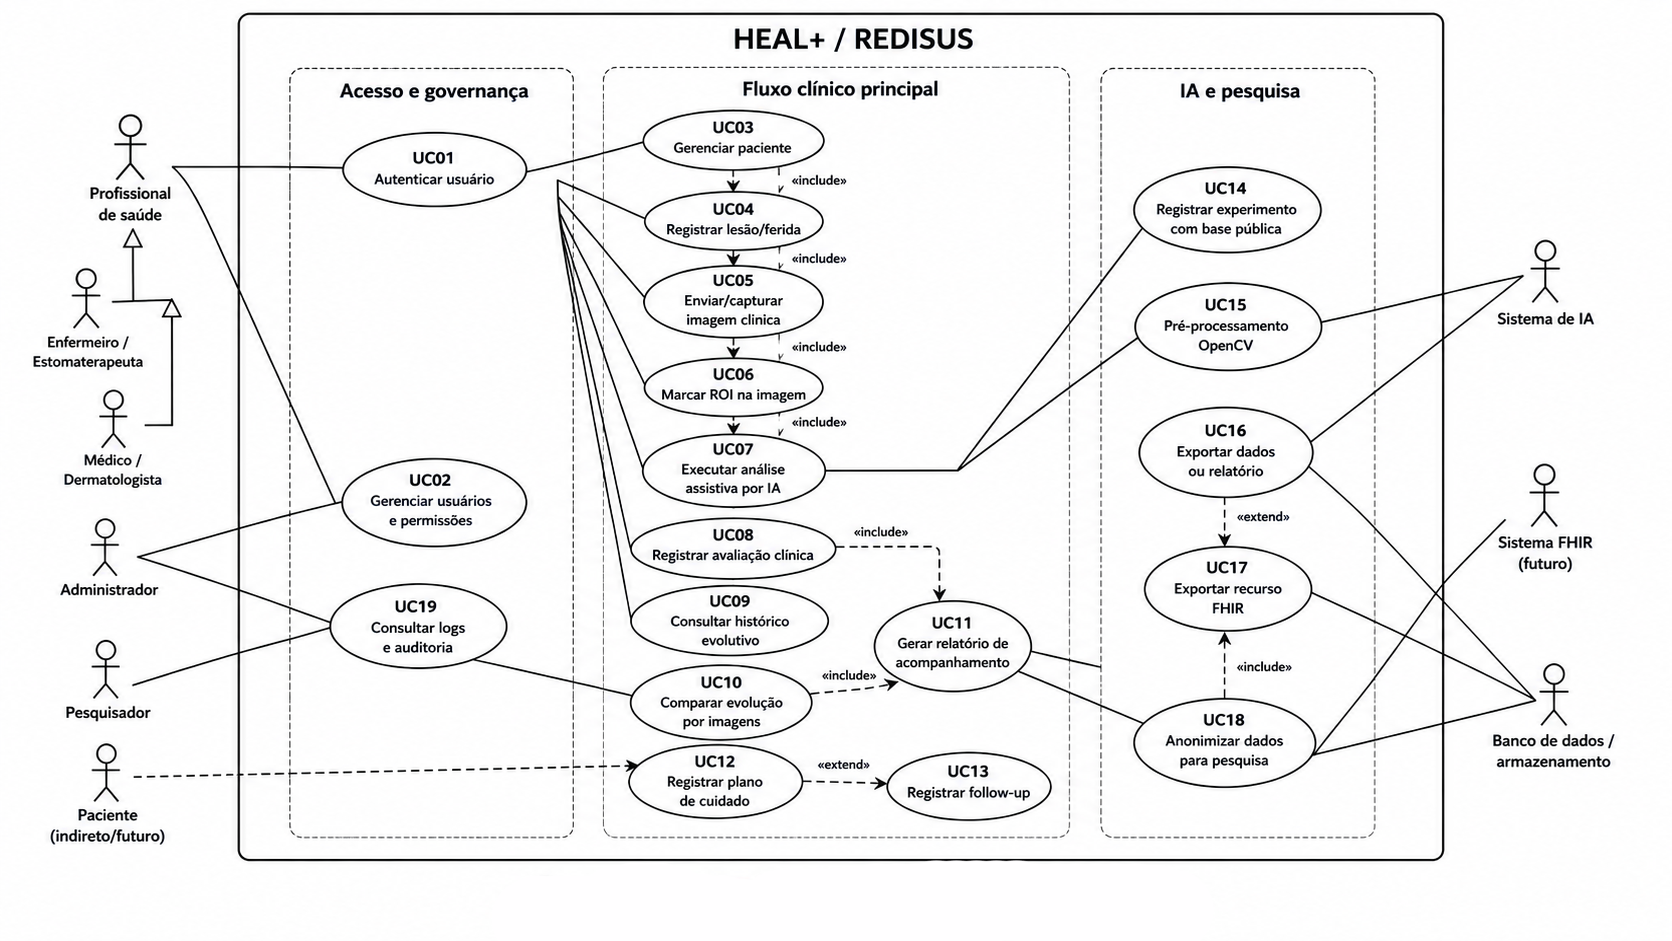
\includegraphics[width=\textwidth,height=0.72\textheight,keepaspectratio]{figures/software/use_case_diagram.png}
    \caption{\label{fig:diagrama-casos-uso}Diagrama geral de casos de uso do HEAL+ / REDISUS}
    \fonte{Elaboração própria, com base na modelagem funcional do projeto.}
\end{figure}

\begin{figure}[htbp]
    \centering
    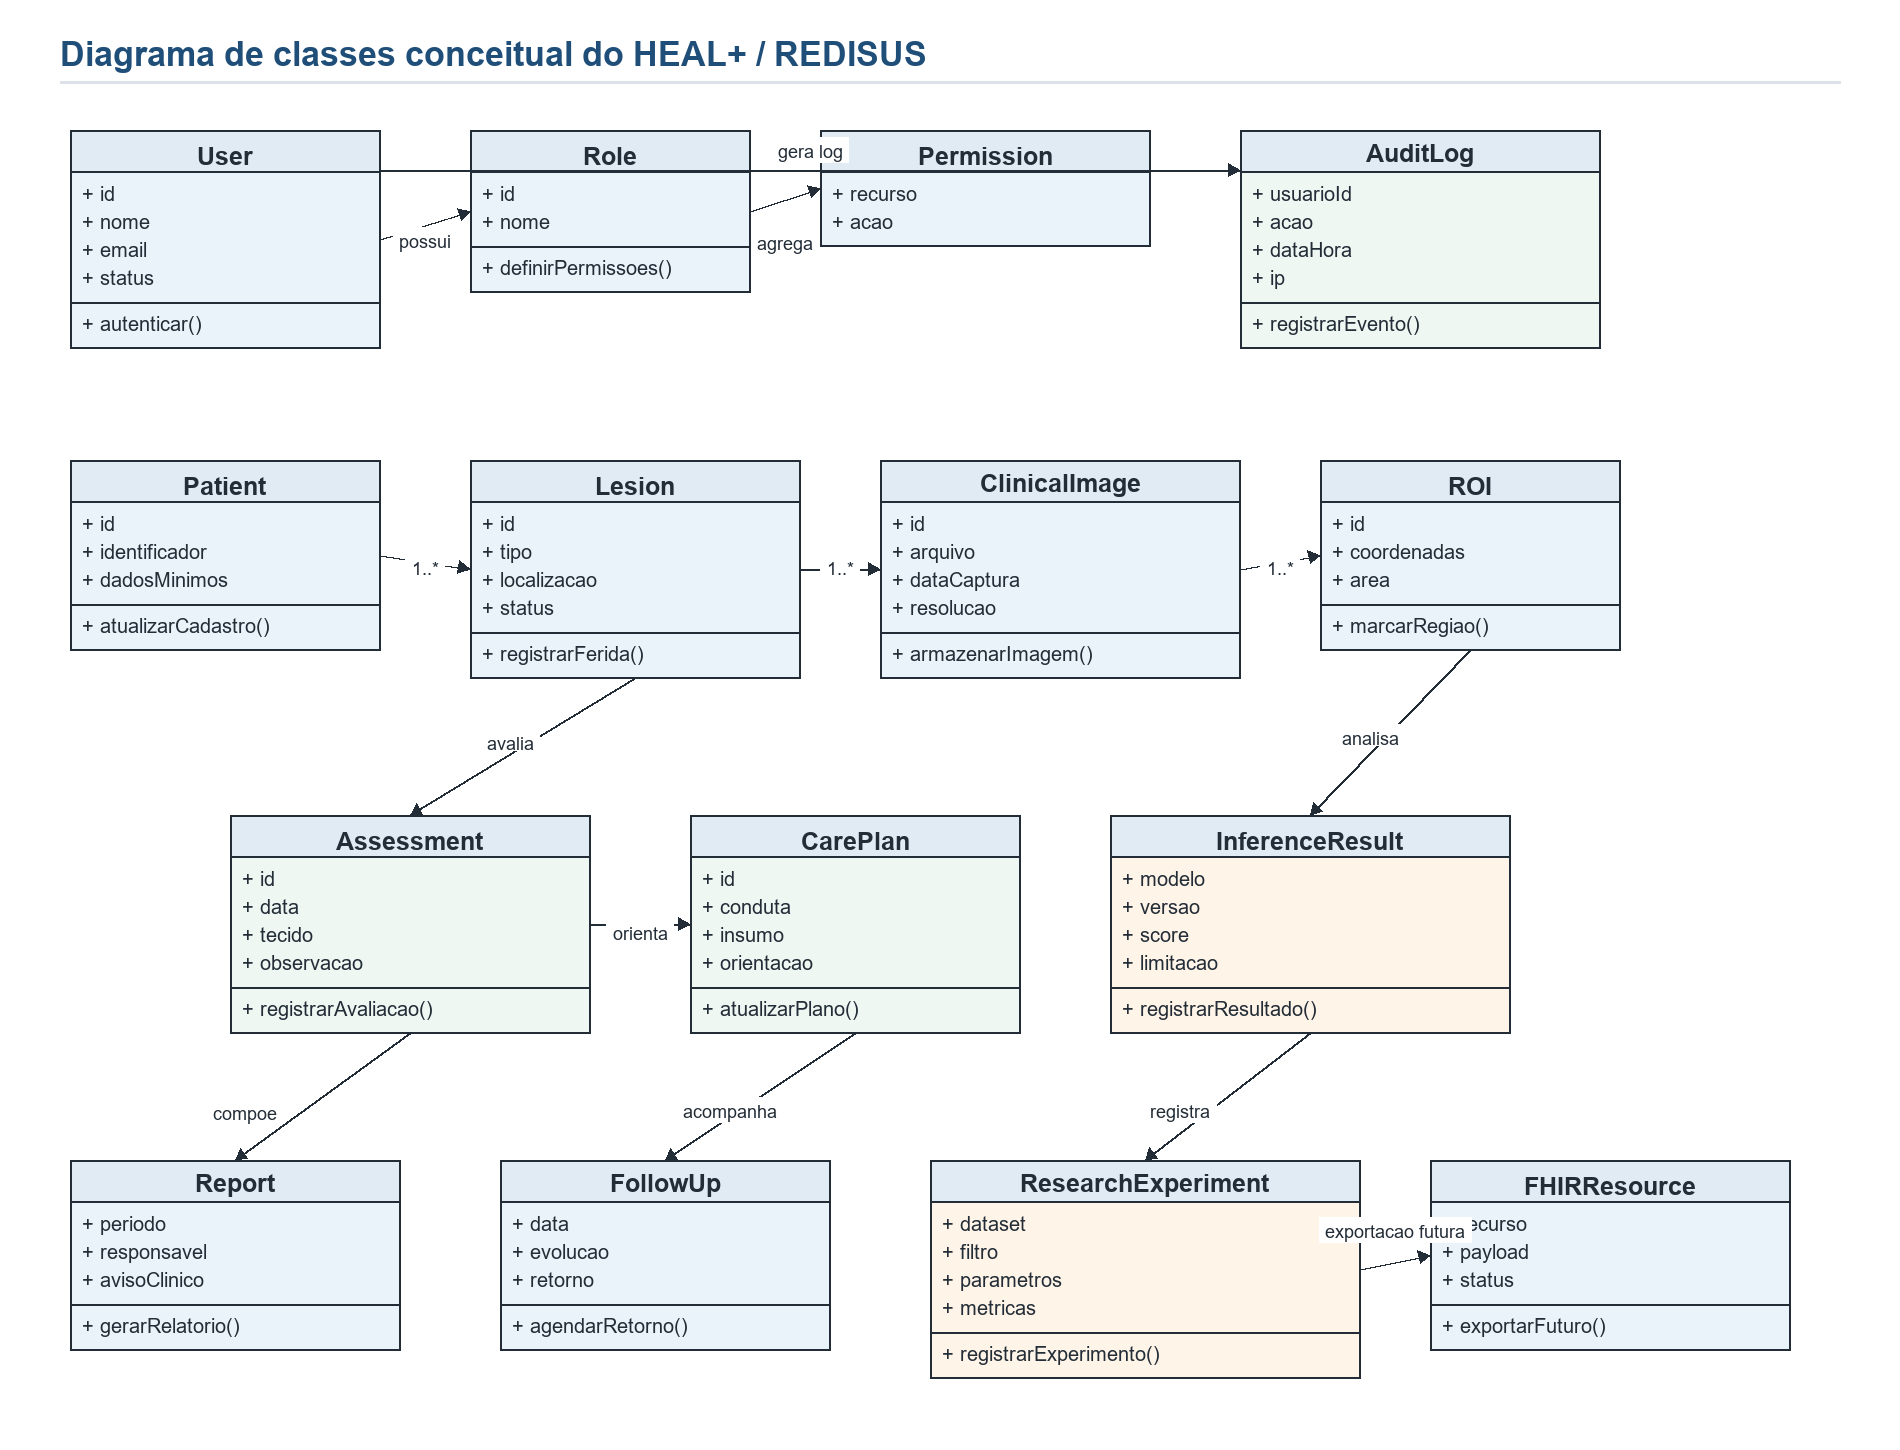
\includegraphics[width=\textwidth,height=0.72\textheight,keepaspectratio]{figures/software/class_diagram.png}
    \caption{\label{fig:diagrama-classes}Diagrama de classes conceitual do HEAL+ / REDISUS}
    \fonte{Elaboração própria, com base na modelagem estrutural da solução.}
\end{figure}

\begin{figure}[htbp]
    \centering
    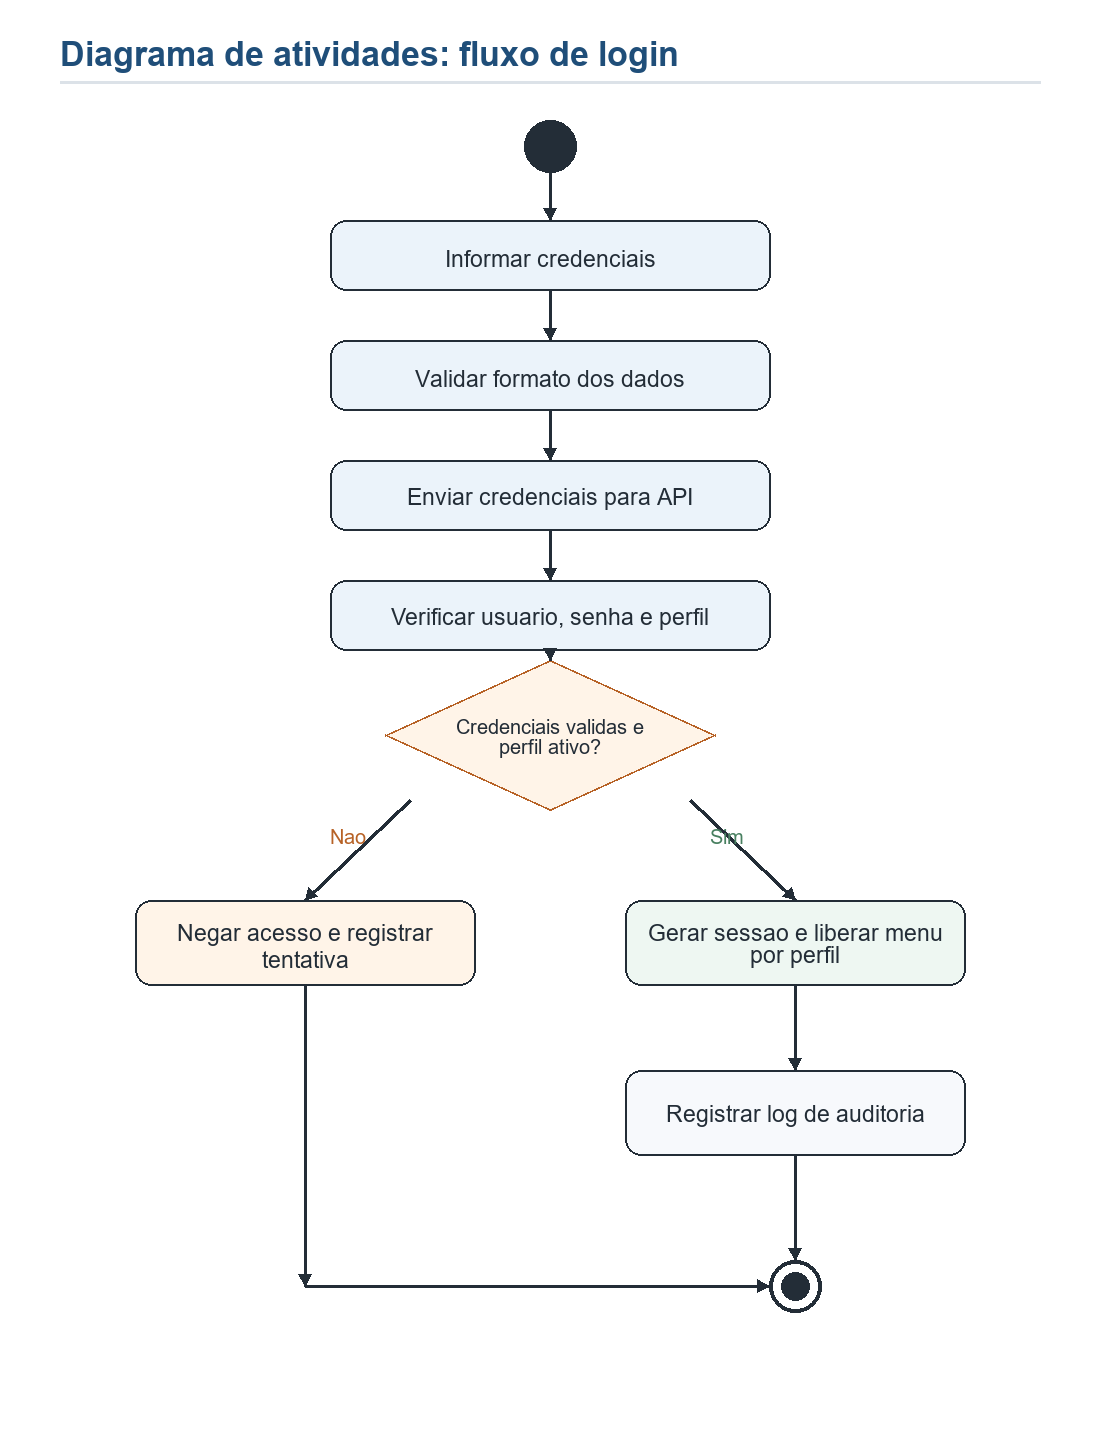
\includegraphics[width=\textwidth,height=0.72\textheight,keepaspectratio]{figures/software/activity_login.png}
    \caption{\label{fig:atividade-login}Diagrama de atividades do fluxo de login}
    \fonte{Elaboração própria.}
\end{figure}

\begin{figure}[htbp]
    \centering
    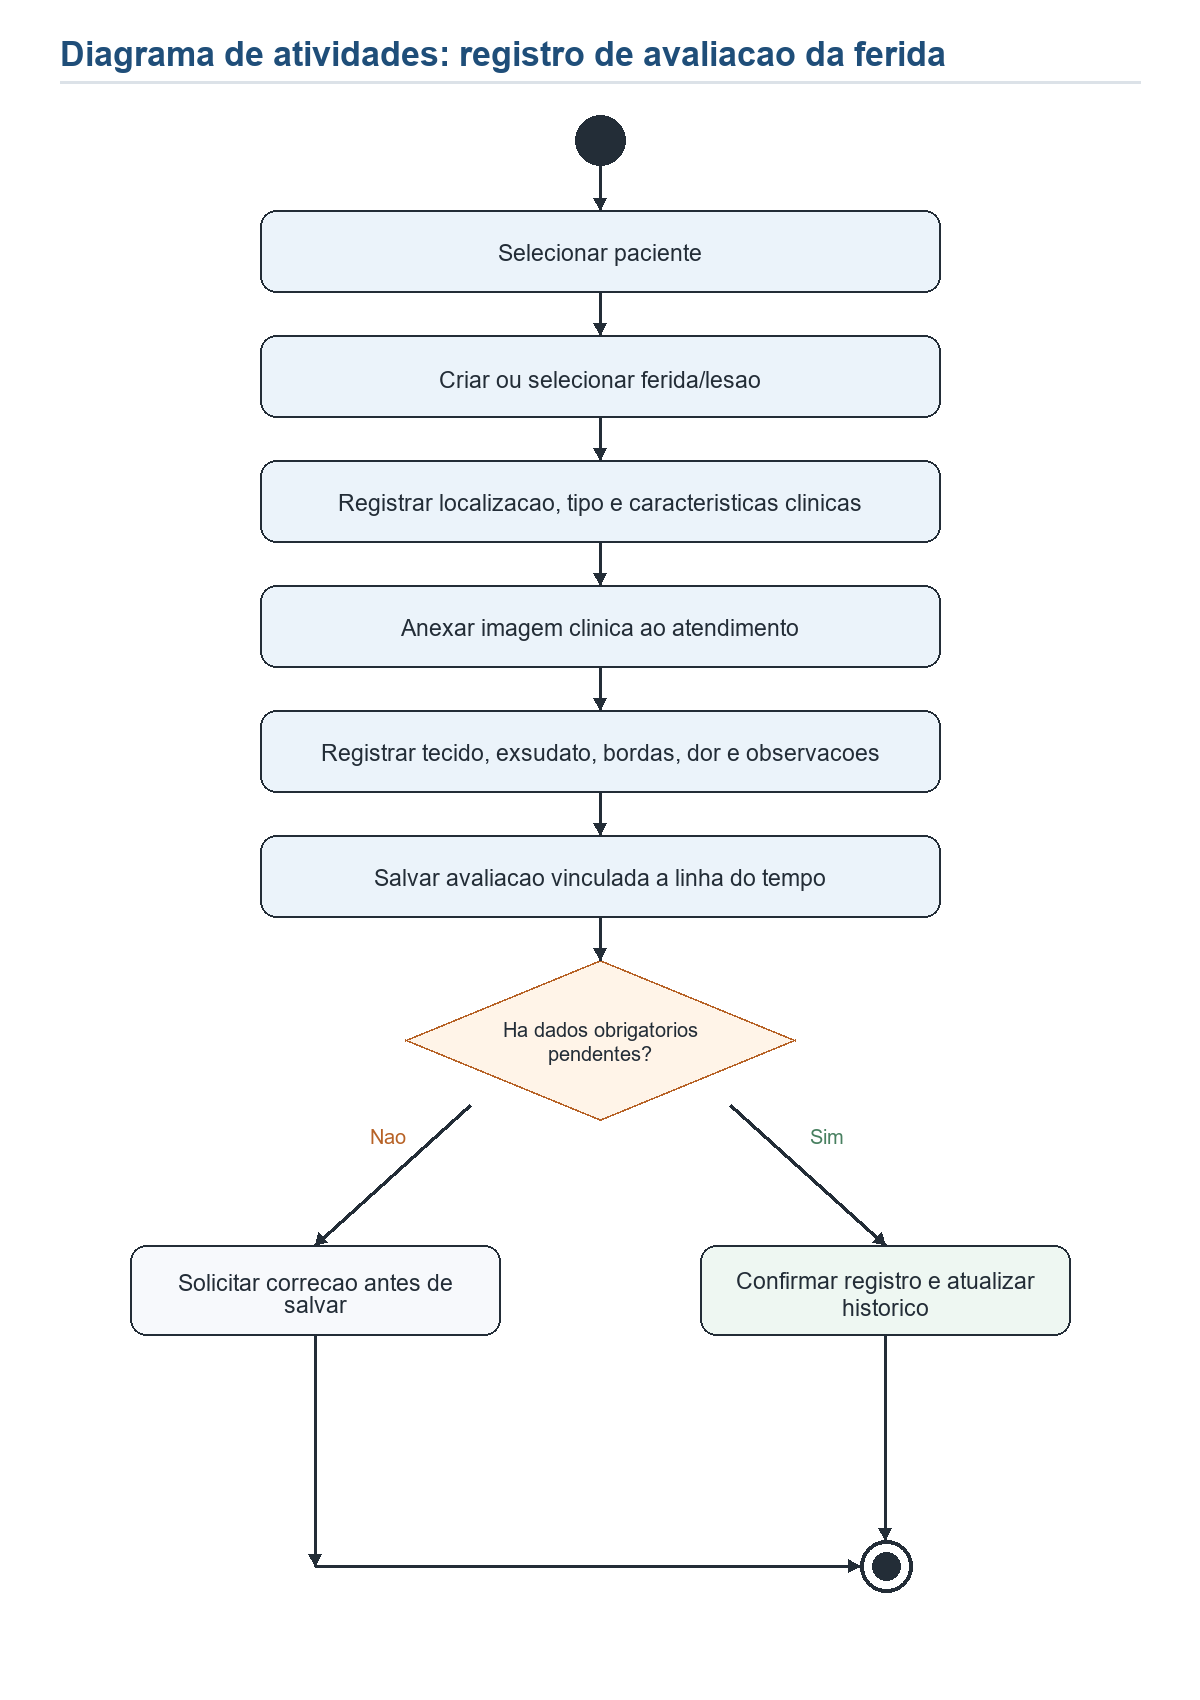
\includegraphics[width=\textwidth,height=0.72\textheight,keepaspectratio]{figures/software/activity_assessment.png}
    \caption{\label{fig:atividade-avaliacao-ferida}Diagrama de atividades do registro de avaliação da ferida}
    \fonte{Elaboração própria.}
\end{figure}

\begin{figure}[htbp]
    \centering
    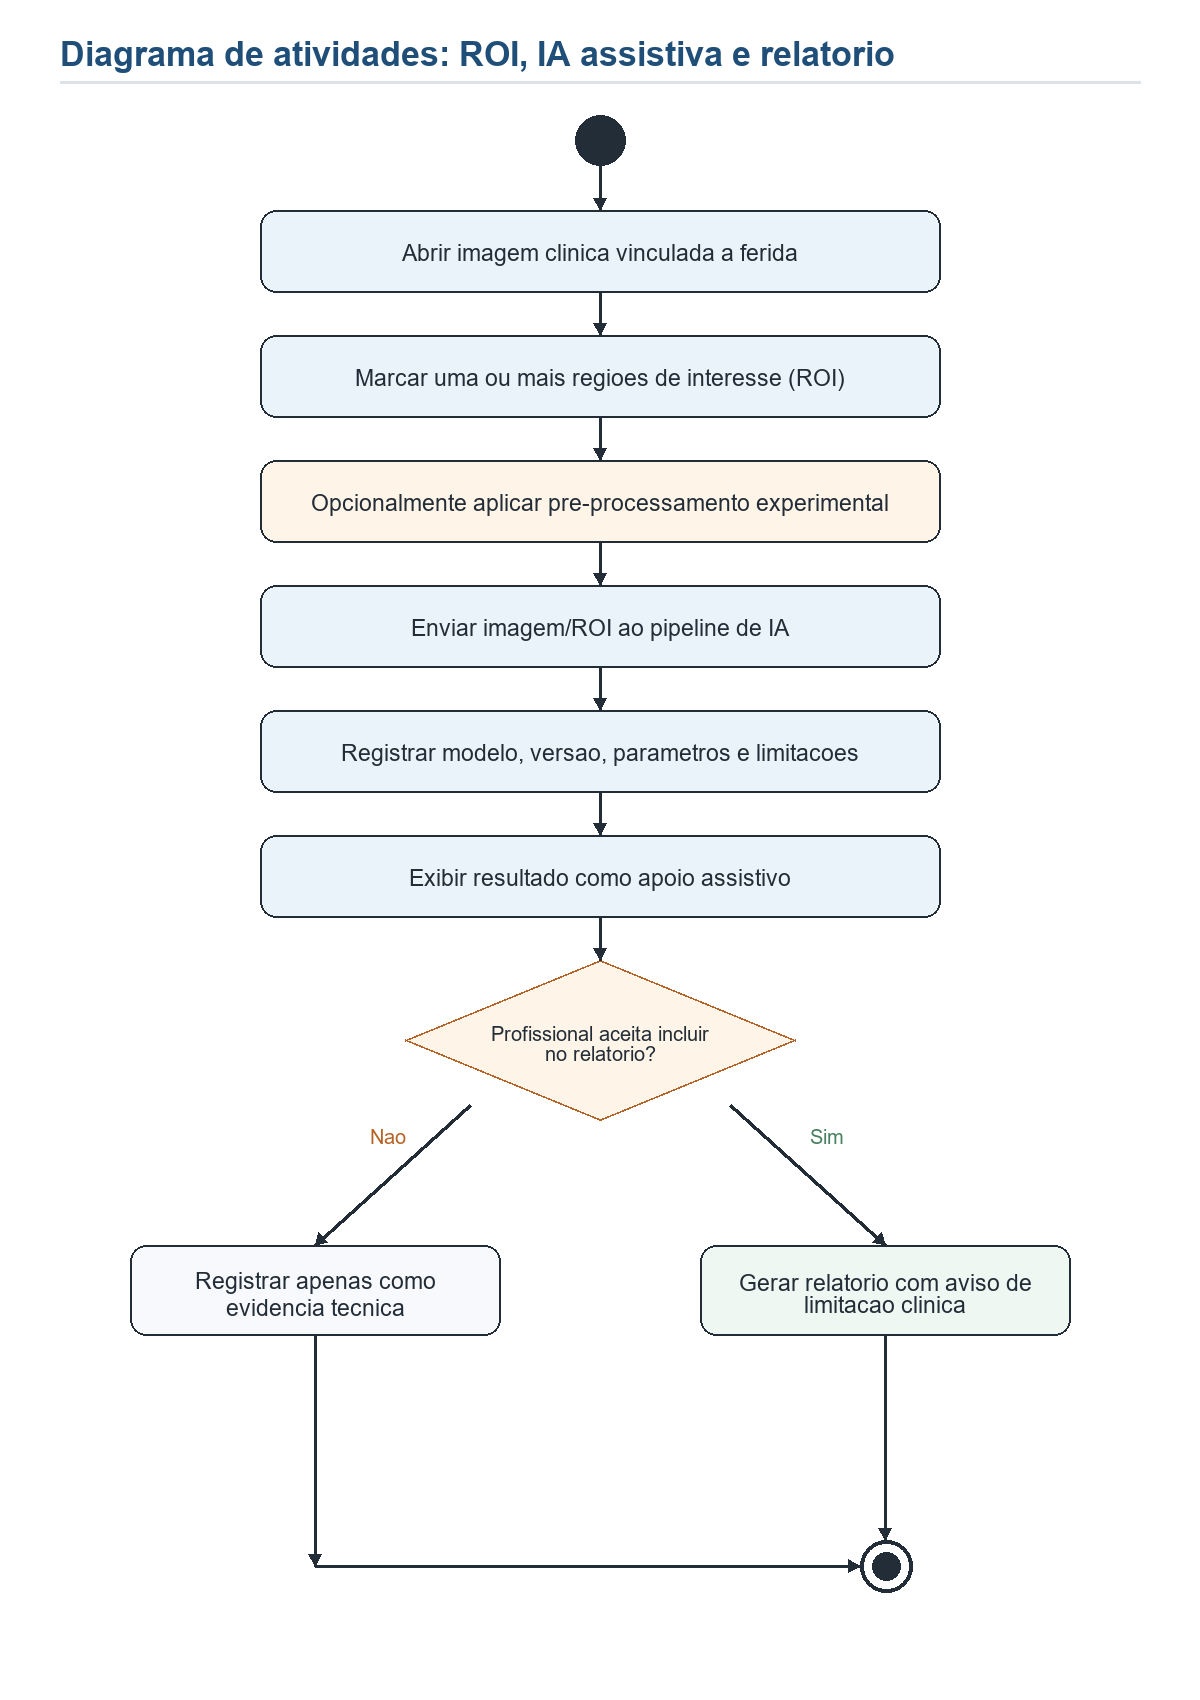
\includegraphics[width=\textwidth,height=0.72\textheight,keepaspectratio]{figures/software/activity_roi_ai_report.png}
    \caption{\label{fig:atividade-roi-ia-relatorio}Diagrama de atividades do fluxo de ROI, IA assistiva e relatório}
    \fonte{Elaboração própria.}
\end{figure}

\begin{figure}[htbp]
    \centering
    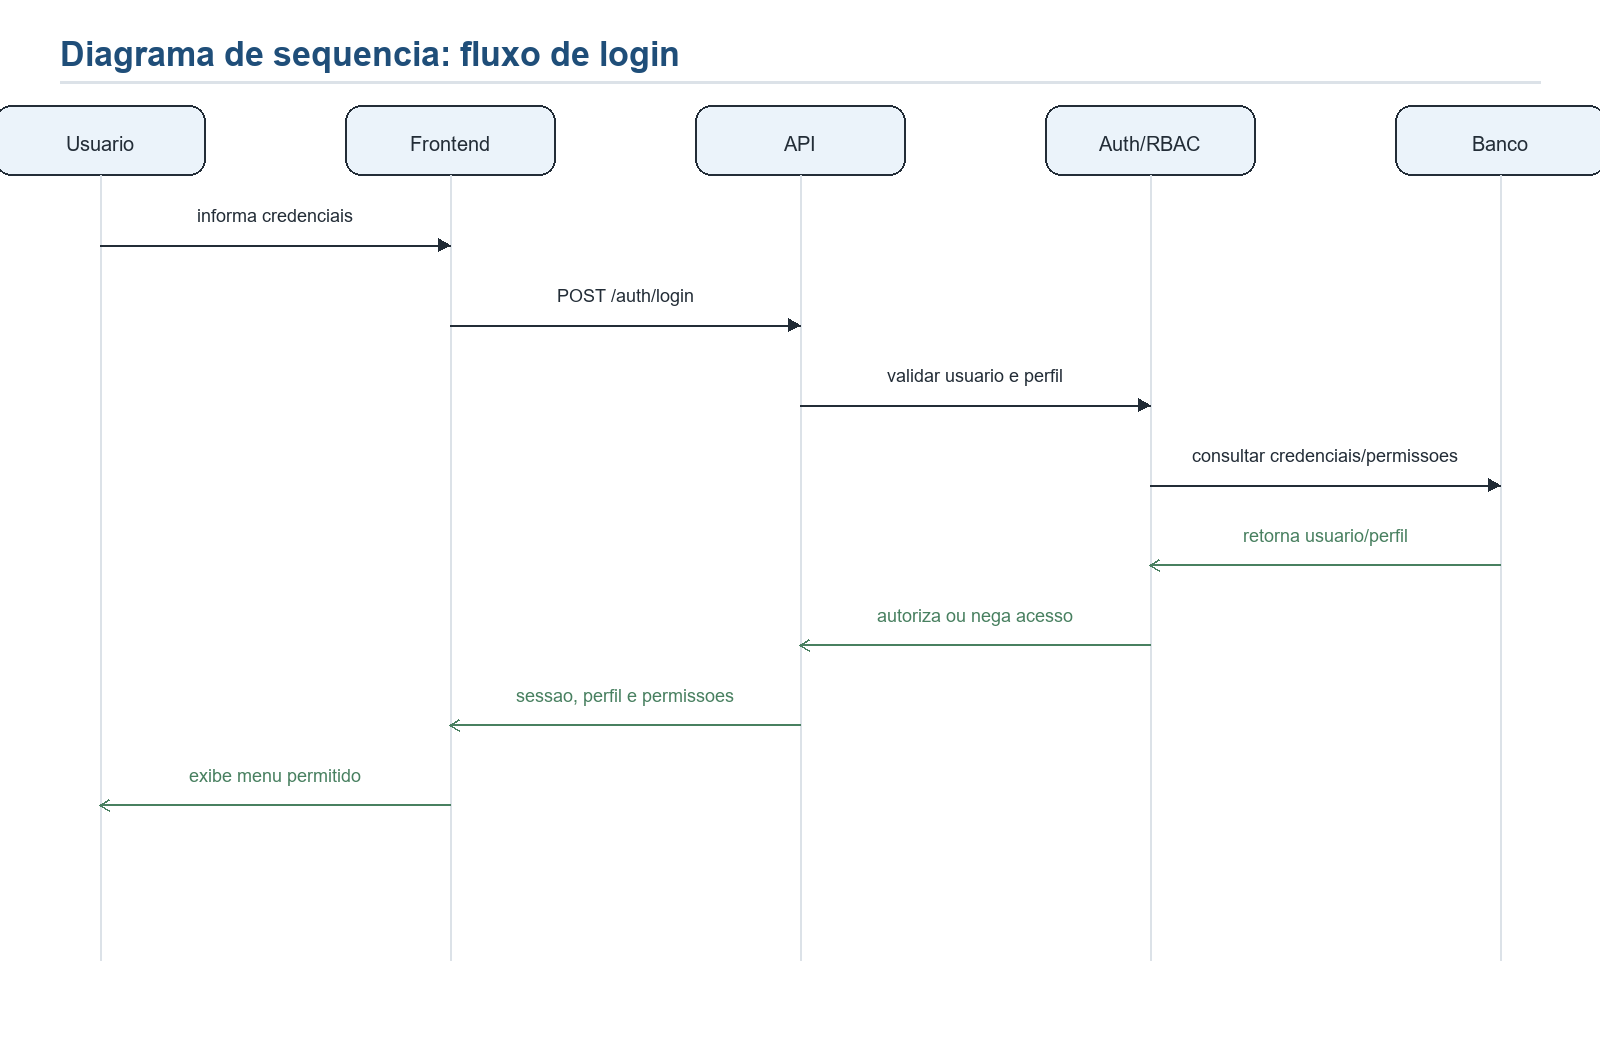
\includegraphics[width=\textwidth,height=0.72\textheight,keepaspectratio]{figures/software/sequence_login.png}
    \caption{\label{fig:sequencia-login}Diagrama de sequência do fluxo de login}
    \fonte{Elaboração própria.}
\end{figure}

\begin{figure}[htbp]
    \centering
    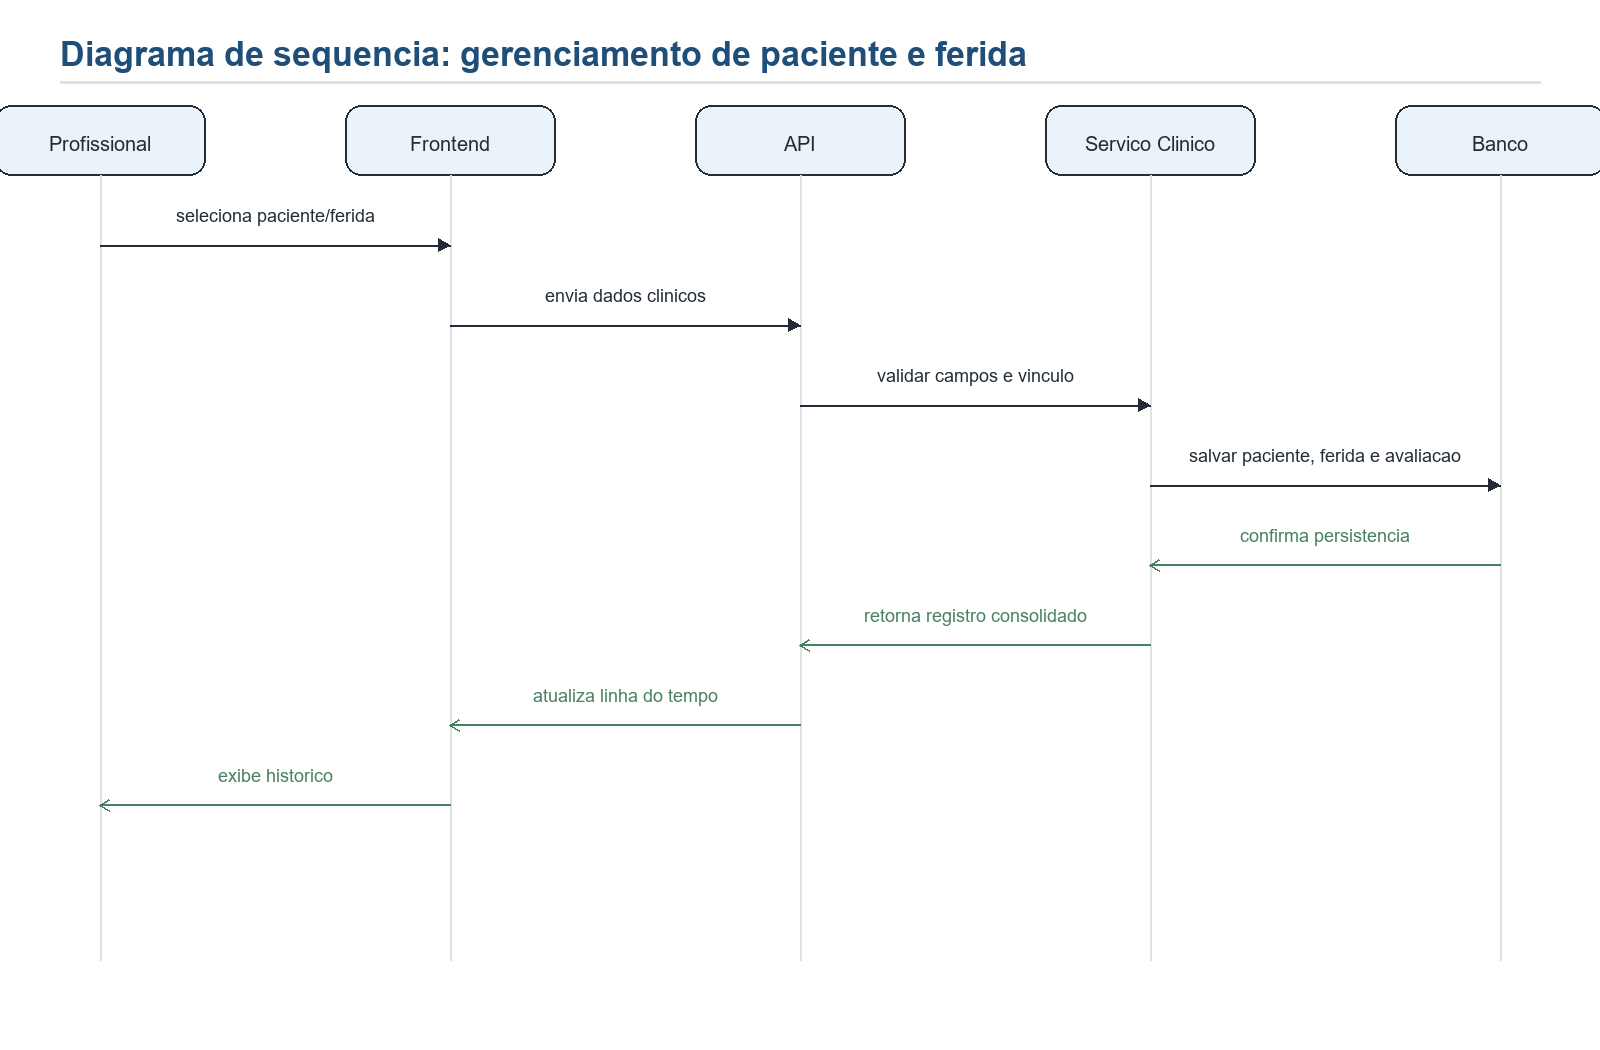
\includegraphics[width=\textwidth,height=0.72\textheight,keepaspectratio]{figures/software/sequence_patient_wound.png}
    \caption{\label{fig:sequencia-paciente-ferida}Diagrama de sequência do gerenciamento de paciente e ferida}
    \fonte{Elaboração própria.}
\end{figure}

\begin{figure}[htbp]
    \centering
    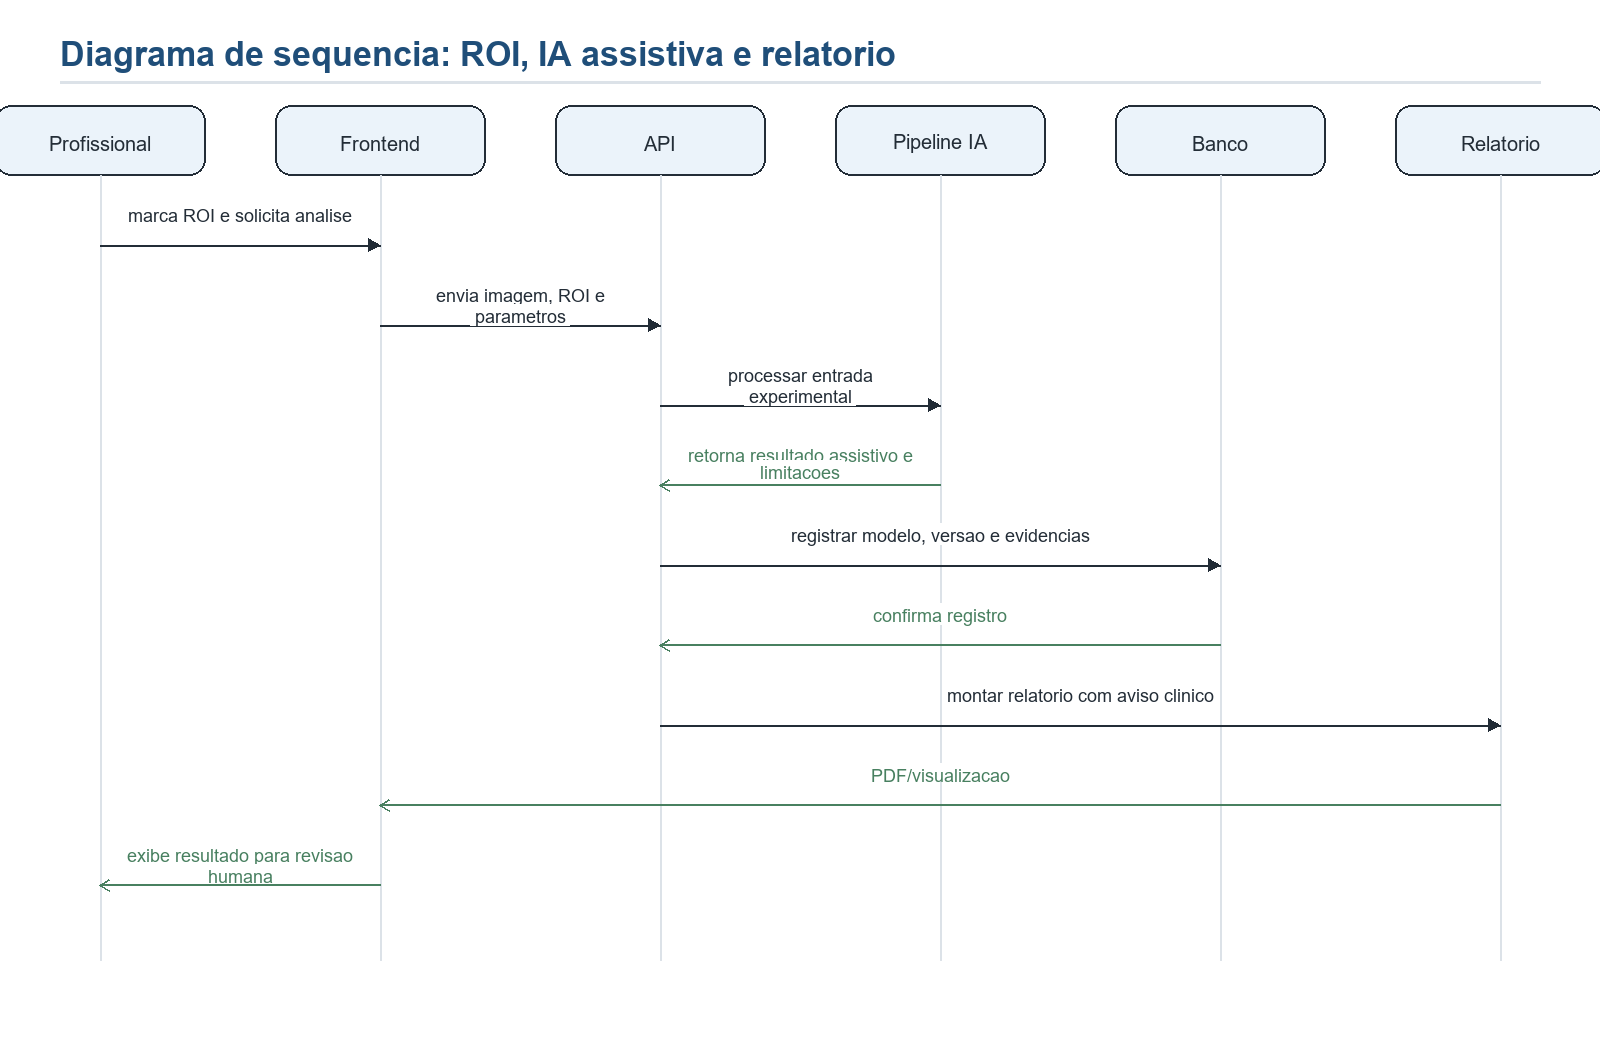
\includegraphics[width=\textwidth,height=0.72\textheight,keepaspectratio]{figures/software/sequence_roi_ai_report.png}
    \caption{\label{fig:sequencia-roi-ia-relatorio}Diagrama de sequência do fluxo de ROI, IA assistiva e relatório}
    \fonte{Elaboração própria.}
\end{figure}

\begin{figure}[htbp]
    \centering
    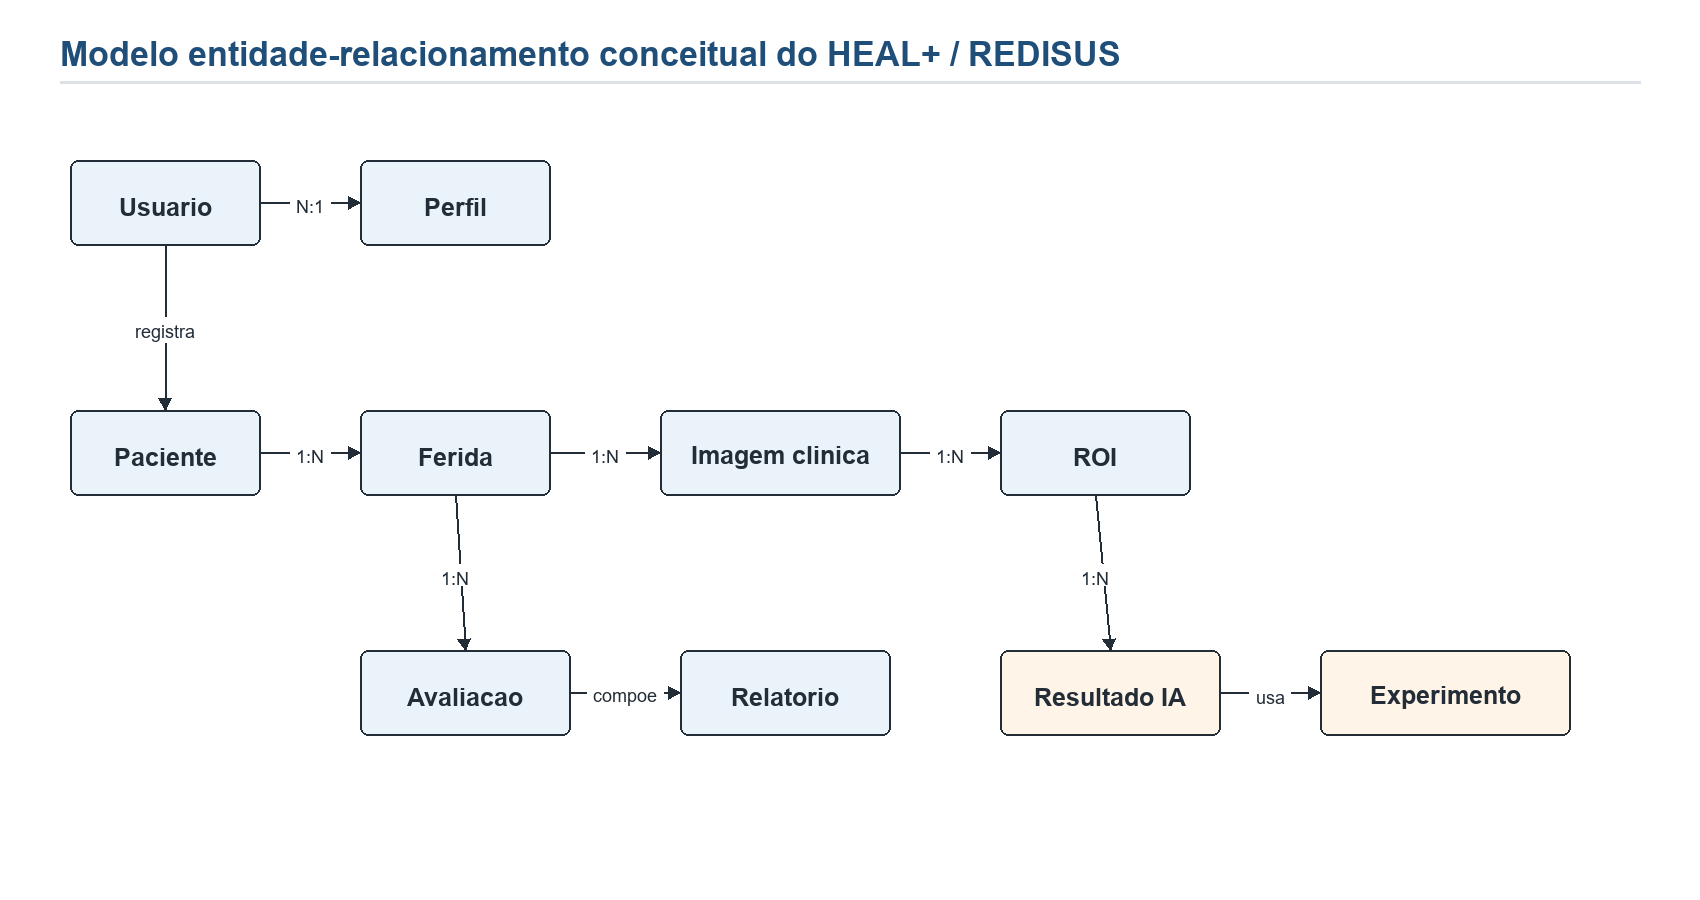
\includegraphics[width=\textwidth,height=0.62\textheight,keepaspectratio]{figures/software/conceptual_er.png}
    \caption{\label{fig:modelo-er-conceitual}Modelo entidade-relacionamento conceitual do HEAL+ / REDISUS}
    \fonte{Elaboração própria, com base na modelagem conceitual dos dados do projeto.}
\end{figure}

\clearpage

\section{Relação entre modelagem, requisitos e rastreabilidade}

A modelagem proposta fortalece a matriz de rastreabilidade porque associa requisitos funcionais, regras de negócio, atores e evidências visuais. Essa relação auxilia a verificar se funcionalidades críticas possuem representação no fluxo da solução e se há coerência entre requisitos, casos de uso, arquitetura conceitual e critérios de validação.

\begin{longtable}{L{4.0cm}L{3.3cm}L{5.7cm}}
\caption{\label{tab:rastreabilidade-casos-uso}Complemento da rastreabilidade com casos de uso e diagramas}\\
\toprule
\textbf{Requisito} & \textbf{Caso de uso relacionado} & \textbf{Evidência de modelagem} \\
\midrule
\endfirsthead
\toprule
\textbf{Requisito} & \textbf{Caso de uso relacionado} & \textbf{Evidência de modelagem} \\
\midrule
\endhead
RF02 -- Login e autenticação & UC01 & Diagrama de atividades e sequência de login; classes User, Role, Permission e AuditLog. \\
RF03 -- Cadastro de pacientes & UC03 & Sequência de gerenciamento de paciente e entidade Patient. \\
RF05 -- Registro de feridas & UC04 & Classe Lesion, fluxo de avaliação e entidade Ferida. \\
RF06 -- Upload de imagens & UC05 & Classe ClinicalImage e vínculo com Ferida. \\
RF07 -- Marcação de ROI & UC06 & Classe ROI, atividade de ROI e análise assistiva. \\
RF10 -- Relatório de acompanhamento & UC11 & Classe Report e sequência de ROI, IA e relatório. \\
RF14 -- Controle de permissões & UC02 & Relação entre User, Role e Permission. \\
RF16 -- Testes com bases públicas & UC14 & ResearchExperiment e separação entre uso experimental e assistencial. \\
RF17 -- Registro de métricas de IA & UC14, UC15 & InferenceResult e ResearchExperiment. \\
RF19 -- Log de auditoria & UC01, UC02, UC19 & Classe AuditLog e fluxo de autenticação. \\
RF20 -- Anonimização para pesquisa & UC18 & Caso de uso de anonimização e preparação ética para pesquisa. \\
\bottomrule
\end{longtable}
\fonte{Elaboração própria.}

\chapter{Testes com bancos de imagens públicos}

O uso de bancos públicos de imagens deve ocorrer em ambiente de pesquisa, respeitando licenças, termos de uso e restrições de redistribuição. O projeto não deve incorporar imagens públicas ao repositório sem autorização. Sempre que possível, os datasets devem permanecer fora do Git e ser referenciados por manifestos, como já previsto pela pasta \texttt{data/manifests/}.

\begin{table}[htbp]
    \centering
    \caption{\label{tab:bases-publicas}Planejamento de testes com imagens públicas}
    \begin{tabular}{L{1.4cm}L{3.2cm}L{4.2cm}L{4.2cm}}
        \toprule
        \textbf{ID} & \textbf{Base ou fonte} & \textbf{Finalidade} & \textbf{Cuidados} \\
        \midrule
        TP01 & PIID & Testar classificação de estágios de lesão por pressão. & Confirmar licença, manter fora do Git quando aplicável e registrar split. \\
        TP02 & Medetec ou equivalente & Testar detecção, organização e preparação para modelos. & Verificar origem, termos e disponibilidade local. \\
        TP03 & Imagens públicas variadas & Avaliar robustez sob diferentes iluminações e ângulos. & Usar apenas material permitido para pesquisa. \\
        TP04 & Subconjunto anotado & Validar ROI, bounding boxes e máscaras. & Registrar anotador, critérios e versão. \\
        TP05 & Base tecidual & Testar segmentação de granulação, esfacelo e necrose. & Padronizar rótulos e revisar clinicamente. \\
        \bottomrule
    \end{tabular}
    \fonte{Elaboração própria.}
\end{table}

Na inspeção local, o conjunto PIID aparece organizado em quatro classes, totalizando 1.091 imagens: 230 de estágio 1, 313 de estágio 2, 275 de estágio 3 e 273 de estágio 4. Esses números correspondem ao acervo local e não devem ser extrapolados para alegações clínicas. O diretório \texttt{dataset/medetec} não continha imagens na inspeção de 5 maio 2026, razão pela qual qualquer afirmação sobre Medetec deve ser verificada com orientação/professor antes de entrar em versão final de submissão.

\chapter{Testes de redimensionamento de imagens para IA}

A análise por imagem depende da qualidade da captura, da padronização da entrada, da ROI e do tamanho usado pelo modelo. Reduções excessivas podem remover bordas finas, tecidos pequenos, variações de cor e características perilesionais; imagens grandes elevam custo computacional e podem dificultar uso em dispositivos modestos \cite{anisuzzaman2022,dabas2023}.

A análise técnica de sensibilidade à resolução espacial avaliou o conjunto PIID no split de teste de 165 imagens. O experimento degradou imagens para diferentes resoluções e reamostrou para 224 x 224, comparando a saída degradada com a referência interna do próprio pipeline clássico. O menor ponto que satisfez simultaneamente os critérios internos foi 80 x 80 para o pipeline clássico; contudo, o mínimo operacional recomendado para o sistema unificado permanece 224 x 224, pois o classificador especializado local registra entrada de 224 x 224 e modelos profundos exigem entrada padronizada.

\begin{figure}[htbp]
    \centering
    \begin{tikzpicture}[
        stage/.style={rectangle, rounded corners=2pt, draw=healgreen, fill=heallight, text width=3.0cm, minimum height=1.0cm, align=center, font=\small},
        note/.style={rectangle, rounded corners=2pt, draw=healgray!55, fill=white, text width=3.0cm, minimum height=0.85cm, align=center, font=\scriptsize},
        arrow/.style={-Latex, thick, draw=healgray},
        node distance=0.85cm and 0.8cm
    ]
        \node[stage] (orig) {Imagem original\\ou ROI};
        \node[stage, right=of orig] (resize) {Padronização\\224 x 224};
        \node[stage, right=of resize] (model) {Análise assistiva\\ou pipeline clássico};
        \node[note, below=of orig] (q1) {Qualidade da captura\\e recorte};
        \node[note, below=of resize] (q2) {Versão do modelo\\e resolução usada};
        \node[note, below=of model] (q3) {Métrica, limitação\\e interpretação};
        \node[stage, below=1.05cm of q2] (audit) {Registro\\das evidências};
        \draw[arrow] (orig) -- (resize);
        \draw[arrow] (resize) -- (model);
        \draw[arrow] (orig) -- (q1);
        \draw[arrow] (resize) -- (q2);
        \draw[arrow] (model) -- (q3);
        \draw[arrow] (q1) |- (audit);
        \draw[arrow] (q2) -- (audit);
        \draw[arrow] (q3) |- (audit);
    \end{tikzpicture}
    \caption{\label{fig:redimensionamento}Representação metodológica do redimensionamento e registro de evidências}
    \fonte{Elaboração própria, sem uso de imagem clínica real.}
\end{figure}

\begin{table}[htbp]
    \centering
    \caption{\label{tab:redimensionamento}Síntese interpretativa do redimensionamento}
    \begin{tabular}{L{3.0cm}L{5.0cm}L{5.0cm}}
        \toprule
        \textbf{Resolução} & \textbf{Uso interpretado} & \textbf{Cautela} \\
        \midrule
        224 x 224 & Mínimo operacional recomendado para sistema unificado. & Adequado à configuração local do classificador PIID. \\
        96 x 96 a 224 x 224 & Faixa estável para análise clássica no experimento local. & Não substitui validação por especialista. \\
        80 x 80 & Mínimo técnico interno do pipeline clássico testado. & Não recomendado como padrão operacional para IA profunda. \\
        Abaixo de 64 x 64 & Faixa de degradação crescente. & Evitar para decisão técnica, salvo teste controlado. \\
        \bottomrule
    \end{tabular}
    \fonte{Elaboração própria, a partir da análise técnica de resolução espacial do projeto.}
\end{table}

\section{Pré-processamento experimental com OpenCV}

Atendendo à orientação da professora Márcia, foi acrescentada uma etapa experimental de pré-processamento de imagens com OpenCV antes da análise pelo HEAL+. Essa etapa não substitui o pipeline principal e deve ser usada apenas para comparação controlada. As funções foram organizadas em \texttt{src/processing/preprocessing\_filters.py} e o script de execução em \texttt{scripts/run\_preprocessing\_experiments.py}.

Foram implementados filtro passa-baixa por mediana com \texttt{cv2.medianBlur()}, filtro passa-baixa gaussiano com \texttt{cv2.GaussianBlur()}, equalização global de histograma em escala de cinza com \texttt{cv2.equalizeHist()}, equalização de luminância em imagem colorida por YCrCb, CLAHE em luminância por LAB e combinações entre filtro e equalização. A equalização colorida foi aplicada apenas no canal de luminância para reduzir distorção cromática da ferida.

O script gera dez variantes: original, mediana, gaussiana, equalização em cinza, equalização colorida, CLAHE colorido, mediana com equalização, gaussiano com equalização, mediana com CLAHE e gaussiano com CLAHE. Para cada variante, salva imagem processada, linha em CSV comparativo e grade visual na pasta de relatórios do experimento. Métricas inexistentes no pipeline são registradas como \texttt{not\_available}, sem inferência manual de resultados.

Como verificação inicial, o script foi executado em 5 maio 2026 sobre a imagem sintética \texttt{examples/synthetic\_wound.jpg}, sem uso de imagem real de paciente. No ambiente local de teste, alguns modelos profundos opcionais não estavam carregados por ausência de dependências ou pesos, de modo que os valores abaixo representam apenas uma execução técnica de fumaça do analisador clínico disponível, não validação clínica.

\begin{table}[htbp]
    \centering
    \caption{\label{tab:opencv-preprocessamento}Execução inicial dos filtros OpenCV em imagem sintética}
    \begin{tabular}{L{4.0cm}C{2.6cm}C{2.1cm}L{4.0cm}}
        \toprule
        \textbf{Método} & \textbf{Área detectada} & \textbf{ROI} & \textbf{Observação} \\
        \midrule
        Original & 53.823 px & 1 & Ferida válida; tecido predominante: esfacelo. \\
        Mediana & 55.209 px & 1 & Alterou discretamente a área detectada. \\
        Gaussiano & 55.902 px & 1 & Alterou discretamente a área detectada. \\
        Equalização em cinza & 0 px & não disponível & Rejeitada pelo analisador por perda de características cromáticas. \\
        Equalização colorida & 307.200 px & 1 & Expansão excessiva da área detectada no teste sintético. \\
        CLAHE colorido & 37.356 px & 1 & Reduziu a área detectada em relação ao original. \\
        Mediana + equalização & 307.200 px & 1 & Expansão excessiva da área detectada no teste sintético. \\
        Gaussiano + equalização & 307.200 px & 1 & Expansão excessiva da área detectada no teste sintético. \\
        Mediana + CLAHE & 37.211 px & 1 & Resultado próximo ao CLAHE colorido. \\
        Gaussiano + CLAHE & 41.148 px & 1 & Resultado intermediário entre CLAHE e original. \\
        \bottomrule
    \end{tabular}
    \fonte{Elaboração própria, a partir de execução experimental sobre imagem sintética do repositório.}
\end{table}

Esses resultados iniciais indicam que o pré-processamento pode alterar significativamente a área detectada e a aceitação da imagem pelo analisador. A equalização em escala de cinza, por remover a informação de cor, foi rejeitada na verificação sintética; já a equalização global colorida ampliou excessivamente a área detectada. Esse comportamento reforça que filtros devem ser avaliados empiricamente, imagem a imagem, antes de qualquer adoção operacional. Não se conclui, nesta etapa, que qualquer filtro melhora a IA.

\chapter{Uso de ROI}

A ROI, ou região de interesse, reduz interferências externas à ferida, como pele saudável, curativos, sombras, fundo, objetos e múltiplas lesões no mesmo enquadramento. Em imagens clínicas, a delimitação manual ou assistida ajuda a concentrar o processamento na área relevante e se relaciona diretamente com segmentação, mensuração e classificação \cite{anisuzzaman2022,dabas2023}.

No estado atual do projeto, o README e as rotas de integração descrevem etapa manual obrigatória de ROI no analisador web, com polígono, desenho livre, círculo e suporte a múltiplas ROIs por imagem. Essas ROIs são convertidas em máscaras binárias e utilizadas como filtro principal para validação, segmentação, tecidos e sobreposições visuais.

\begin{figure}[htbp]
    \centering
    \begin{tikzpicture}[
        box/.style={rectangle, rounded corners=2pt, draw=healblue, fill=heallight, minimum width=2.8cm, minimum height=0.8cm, align=center, font=\small},
        warn/.style={rectangle, rounded corners=2pt, draw=healorange, fill=healorange!10, minimum width=4.2cm, minimum height=0.8cm, align=center, font=\small},
        arrow/.style={-Latex, thick, draw=healblue}
    ]
        \node[box] (img) {Imagem\\clínica};
        \node[box, right=of img] (roi) {ROI manual\\ou assistida};
        \node[box, right=of roi] (mask) {Máscara e\\metadados};
        \node[box, below=of mask] (ia) {IA ou análise\\exploratória};
        \node[box, left=of ia] (report) {Relatório com\\limitações};
        \node[warn, below=of report] (human) {Supervisão humana obrigatória\\e ausência de diagnóstico autônomo};
        \draw[arrow] (img) -- (roi);
        \draw[arrow] (roi) -- (mask);
        \draw[arrow] (mask) -- (ia);
        \draw[arrow] (ia) -- (report);
        \draw[arrow] (report) -- (human);
    \end{tikzpicture}
    \caption{\label{fig:roi-ia}Fluxo seguro para ROI, análise assistiva e relatório}
    \fonte{Elaboração própria, com base nas diretrizes da OMS para IA em saúde.}
\end{figure}

\chapter{Inteligência artificial e visão computacional}

O HEAL+ prevê uso de IA e visão computacional para apoiar análise de feridas, porém esses recursos devem permanecer em estágio experimental até validação adequada. A implementação atual inclui pipeline de inferência, segmentação tecidual clássica, classificadores experimentais, model card de lesão por pressão, registro de modelos e documentação de limitações.

O model card do classificador de lesão por pressão informa uso de ResNet50, dataset PIID local, entrada 224 x 224, quatro classes de estágio, split de 763 imagens de treino, 163 de validação e 165 de teste, além de acurácia de teste de 0,7030 no baseline inicial. Esses valores devem ser descritos apenas como resultados exploratórios locais, pois não equivalem a validação clínica externa nem autorizam uso autônomo para estadiamento.

Toda saída de IA deve conter: data, versão do modelo, dataset, split, métrica, confiança ou incerteza, limitações, indicação de supervisão humana, vínculo entre imagem e ROI, e aviso de que a interpretação final é profissional. Recomenda-se ainda registrar exemplos de falha, análise de viés, qualidade da imagem e critérios de revisão por especialista.

\chapter{Aspectos éticos}

O HEAL+ lida com dados de saúde e imagens clínicas, por isso aspectos éticos devem orientar o projeto desde a concepção. A Resolução CNS nº 466/2012 estabelece diretrizes para pesquisas envolvendo seres humanos, incluindo respeito à dignidade, autonomia, beneficência, não maleficência, justiça, equidade, consentimento e análise de riscos e benefícios \cite{brasil2012}. A Resolução CNS nº 510/2016 deve ser considerada quando a pesquisa envolver Ciências Humanas e Sociais, dados diretamente obtidos de participantes ou informações identificáveis \cite{brasil2016}.

Qualquer coleta, armazenamento, análise ou compartilhamento de imagens reais de pacientes para pesquisa deve ser submetido ao CEP antes de execução. Enquanto não houver aprovação ética, os testes devem se limitar a dados sintéticos, imagens públicas permitidas ou bases licenciadas. O protocolo deve explicar se haverá IA, quais dados serão processados, como serão protegidos, quais riscos existem e que o sistema não será usado para decisão clínica autônoma \cite{who2021,brasil2012}.

As figuras metodológicas foram criadas como diagramas esquemáticos, sem uso de fotografia clínica real. Essa decisão reduz risco de exposição indevida e evita inserir imagem sensível sem comprovação de TCLE, anonimização e aprovação ética.

\chapter{LGPD e proteção de dados}

A LGPD estabelece regras para tratamento de dados pessoais e sensíveis. No HEAL+, dados de pacientes, fotografias de feridas, relatórios e histórico de acompanhamento devem ser tratados como informações sensíveis e protegidos por medidas técnicas e administrativas \cite{brasil2018,anpd2023}. A classificação interna do projeto trata imagens de feridas, dados clínicos, relatórios estruturados e histórico de atendimento como sensíveis críticos.

As diretrizes mínimas são: coletar apenas dados necessários; informar finalidade; restringir acesso por perfil; registrar logs; evitar dados reais em ambiente de teste; anonimizar ou pseudonimizar dados de pesquisa; armazenar imagens com segurança; não compartilhar com terceiros sem base legal ou autorização; definir retenção e descarte; e manter documentação de governança.

\chapter{Preparação para submissão ao CEP}

A submissão ao CEP será necessária caso o projeto envolva coleta, uso, análise, armazenamento ou compartilhamento de dados e imagens reais de pacientes em pesquisa. A preparação deve incluir título, pesquisadores responsáveis, instituição proponente, justificativa, objetivos, metodologia, critérios de inclusão e exclusão, dados coletados, riscos, benefícios, TCLE, plano de anonimização, armazenamento, descarte, autorização institucional e explicação sobre IA.

O protocolo deve deixar explícito que o HEAL+ é sistema de apoio ao registro e acompanhamento, não ferramenta autônoma de diagnóstico. Caso modelos de IA sejam avaliados, os resultados devem ser analisados em contexto de pesquisa e comparados com avaliação profissional, sem substituí-la \cite{who2021,who2023,brasil2012}.

\chapter{Riscos}

\begin{longtable}{L{1.5cm}L{3.6cm}L{4.6cm}L{3.6cm}}
\caption{\label{tab:riscos}Riscos do projeto}\\
\toprule
\textbf{ID} & \textbf{Risco} & \textbf{Descrição} & \textbf{Mitigação} \\
\midrule
\endfirsthead
\toprule
\textbf{ID} & \textbf{Risco} & \textbf{Descrição} & \textbf{Mitigação} \\
\midrule
\endhead
R01 & Uso indevido como diagnóstico & Usuário interpretar resultado como diagnóstico definitivo. & Avisos, treinamento e limitação explícita. \\
R02 & Exposição de dados sensíveis & Vazamento de dados ou imagens clínicas. & Controle de acesso, logs, criptografia e minimização. \\
R03 & Uso sem aprovação ética & Pesquisa com imagens reais sem CEP. & Bloquear uso até aprovação. \\
R04 & Viés de dataset & Modelo treinado com base pouco diversa. & Documentar dataset e revisar com especialistas. \\
R05 & Baixa qualidade de imagem & Foco, iluminação ou enquadramento inadequados. & Guia de captura e validação de qualidade. \\
R06 & ROI incorreta & Região marcada não representa a ferida. & Edição, treinamento e revisão profissional. \\
R07 & Métricas superestimadas & Bom resultado interno sem validação externa. & Usar conjunto congelado e evitar claims clínicos. \\
R08 & Perda de dados & Falhas de armazenamento ou backup. & Política de backup e recuperação. \\
R09 & Falha de permissões & Acesso indevido por perfil mal configurado. & RBAC, testes de autorização e auditoria. \\
R10 & Dependência técnica & Dificuldade de manter modelos e bibliotecas. & Versionamento, documentação e ambiente controlado. \\
\bottomrule
\end{longtable}
\fonte{Elaboração própria.}

\chapter{Critérios de validação}

A validação deve ocorrer em camadas: validação técnica do software, validação do fluxo de uso, avaliação com bases públicas, revisão de segurança e privacidade e, apenas após aprovação ética, validação com dados reais de pacientes. Desempenho computacional, usabilidade e validade clínica são dimensões diferentes e não devem ser confundidas \cite{anisuzzaman2022,dabas2023,who2023}.

\begin{table}[htbp]
    \centering
    \caption{\label{tab:validacao}Critérios de validação}
    \begin{tabular}{L{1.4cm}L{3.0cm}L{5.5cm}L{3.2cm}}
        \toprule
        \textbf{ID} & \textbf{Camada} & \textbf{Critério} & \textbf{Evidência} \\
        \midrule
        CV01 & Funcional & Cadastro, edição e consulta funcionam. & Testes automatizados/manuais. \\
        CV02 & Segurança & Acesso restrito por perfil. & Teste de autorização. \\
        CV03 & Usabilidade & Profissional registra ferida sem dificuldade crítica. & Roteiro de teste. \\
        CV04 & Imagens & Upload, vínculo e relatório funcionam. & Casos de teste. \\
        CV05 & ROI & ROI única e múltipla são criadas e editadas. & Teste visual. \\
        CV06 & Relatório & Documento traz dados essenciais e aviso. & PDF/tela. \\
        CV07 & IA experimental & Métricas têm dataset, split e versão. & Relatório de experimento. \\
        CV08 & Ética & Protocolo possui TCLE, riscos e plano de dados. & Checklist CEP. \\
        CV09 & LGPD & Dados sensíveis têm finalidade e acesso restrito. & Revisão documental. \\
        CV10 & Rastreabilidade & Requisito crítico possui teste associado. & Matriz atualizada. \\
        \bottomrule
    \end{tabular}
    \fonte{Elaboração própria.}
\end{table}

\chapter{Cronograma}

\begin{table}[htbp]
    \centering
    \caption{\label{tab:cronograma}Cronograma proposto}
    \begin{tabular}{L{1.3cm}L{5.1cm}L{5.1cm}L{1.6cm}}
        \toprule
        \textbf{Etapa} & \textbf{Atividade} & \textbf{Entregável} & \textbf{Período} \\
        \midrule
        1 & Revisão do escopo e requisitos & Texto do TCC revisado & Mês 1 \\
        2 & Levantamento clínico com profissionais & Campos clínicos validados & Mês 1 \\
        3 & Modelagem de perfis e permissões & Matriz de acesso & Mês 2 \\
        4 & Ajuste do registro de feridas & Protótipo funcional & Mês 2 \\
        5 & Ajuste de imagens e ROI & Fluxo com ROI & Mês 3 \\
        6 & Relatórios e histórico & Relatório de acompanhamento & Mês 3 \\
        7 & Testes com bases públicas & Benchmark exploratório & Mês 4 \\
        8 & Testes de redimensionamento & Comparativo técnico & Mês 4 \\
        9 & Preparação LGPD e CEP & Minuta, TCLE e checklist & Mês 5 \\
        10 & Revisão acadêmica final & TCC consolidado & Mês 6 \\
        \bottomrule
    \end{tabular}
    \fonte{Elaboração própria.}
\end{table}

\chapter{Considerações finais}

O HEAL+ / REDISUS apresenta potencial como módulo de feridas crônicas em uma rede de saúde digital, especialmente por combinar registro estruturado, imagens, ROI, histórico evolutivo, relatórios, rastreabilidade e preparação para IA assistiva. A literatura sustenta a relevância do problema clínico e indica que tecnologias digitais e IA podem contribuir para documentação, mensuração e acompanhamento, desde que submetidas a validação adequada \cite{olsson2019,sen2019,anisuzzaman2022,dabas2023}.

O estudo reforça que o sistema deve ser comunicado como ferramenta de apoio. Ele não substitui diagnóstico, prescrição, estadiamento clínico ou responsabilidade profissional. O uso de IA deve permanecer experimental até que existam validação técnica robusta, validação clínica, governança ética e aprovação pelo CEP quando houver seres humanos \cite{who2021,who2023,brasil2012}.

As próximas etapas recomendadas são: revisar o trabalho com orientador e profissionais da saúde; validar a referência institucional específica do Cluster; confirmar licenças e disponibilidade de bases públicas; amadurecer manifestos de dataset; registrar benchmarks reprodutíveis; preparar minuta de protocolo CEP; e manter a documentação técnica do HEAL+ atualizada durante a evolução do projeto.

\postextual

\bibliographystyle{abntex2-alf}
\bibliography{referencias}

\appendix

\chapter{Checklist inicial para submissão ao CEP}

\begin{enumerate}
    \item Título completo do projeto.
    \item Pesquisador responsável e equipe.
    \item Instituição proponente.
    \item Justificativa científica e social.
    \item Objetivo geral e objetivos específicos.
    \item Descrição detalhada da metodologia.
    \item Critérios de inclusão e exclusão.
    \item Descrição dos dados e imagens coletados.
    \item Riscos e benefícios aos participantes.
    \item Estratégias de minimização de riscos.
    \item Modelo de TCLE.
    \item Plano de anonimização ou pseudonimização.
    \item Plano de armazenamento seguro.
    \item Plano de descarte dos dados.
    \item Autorização institucional, quando aplicável.
    \item Declaração de que o sistema não substitui diagnóstico profissional.
    \item Descrição dos recursos de IA, se houver.
    \item Estratégia de validação e análise dos resultados.
    \item Declaração de uso de IA generativa, quando houver.
\end{enumerate}

\chapter{Modelo de aviso de limitação clínica}

O HEAL+ é uma ferramenta de apoio ao registro, acompanhamento e análise evolutiva de feridas. As informações apresentadas pelo sistema, incluindo imagens, relatórios e eventuais resultados de inteligência artificial, não substituem avaliação, diagnóstico, prescrição, estadiamento ou decisão de profissional de saúde habilitado. Qualquer interpretação clínica deve ser realizada por profissional responsável, considerando o contexto completo do paciente.

\chapter{Dicionário mínimo de dados}

\begin{longtable}{L{3.3cm}L{6.7cm}L{2.2cm}L{1.8cm}}
\caption{\label{tab:dicionario-minimo}Dicionário mínimo de dados}\\
\toprule
\textbf{Campo} & \textbf{Descrição} & \textbf{Tipo} & \textbf{Sensível} \\
\midrule
\endfirsthead
\toprule
\textbf{Campo} & \textbf{Descrição} & \textbf{Tipo} & \textbf{Sensível} \\
\midrule
\endhead
Identificador do paciente & Código interno ou pseudônimo. & Texto/UUID & Sim \\
Nome do paciente & Nome civil, se necessário para uso assistencial. & Texto & Sim \\
Data de nascimento & Informação de identificação e contexto clínico. & Data & Sim \\
Ferida & Identificador da ferida vinculada ao paciente. & Texto/UUID & Sim \\
Localização anatômica & Região corporal da ferida. & Texto & Sim \\
Data da avaliação & Data do registro clínico. & Data & Sim \\
Imagem & Arquivo vinculado à avaliação. & Arquivo & Sim \\
ROI & Coordenadas ou máscara da região de interesse. & JSON & Sim \\
Observação clínica & Texto inserido pelo profissional. & Texto & Sim \\
Conduta e plano de cuidado & Procedimento, curativo, terapia aplicada ou orientação de continuidade. & Texto & Sim \\
Insumos utilizados & Materiais relevantes associados ao atendimento ou procedimento. & Lista & Sim \\
Relatório & Documento gerado pelo sistema. & PDF/HTML & Sim \\
Resultado de IA & Saída experimental de modelo computacional. & JSON & Potencial \\
Log de auditoria & Registro de ação realizada por usuário. & Texto & Sim \\
\bottomrule
\end{longtable}
    \fonte{Elaboração própria.}

\chapter{Template de registro de experimento com IA}

Todo experimento com IA deve registrar, no mínimo:

\begin{itemize}
    \item nome do experimento;
    \item data de execução;
    \item responsável;
    \item objetivo do teste;
    \item dataset utilizado;
    \item licença ou termo de uso do dataset;
    \item versão do dataset;
    \item split de treino, validação e teste;
    \item tamanho das imagens;
    \item modelo utilizado;
    \item parâmetros principais;
    \item métricas obtidas;
    \item limitações observadas;
    \item conclusão;
    \item indicação explícita de que o resultado não possui validação clínica, quando aplicável.
\end{itemize}

\end{document}
